\chapter{METHODOLOGY}
\label{ch:method}

Translating unstructured chief complaints into actionable South African Triage Scale (SATS) classifications requires a rigorous computational pipeline. To bridge the underlying mathematical architecture with its practical application, the following sections employ a recurring illustrative example modeled on a standard patient presentation at \examplehospital{}: \runningcomplaint{} This end-to-end transformation applies to all textual inputs that successfully clear the clinical relevance gate detailed in Section~\ref{sec:gate}. Crucially, this architecture operates strictly as a clinical decision-support mechanism. It provides probabilistic routing guidance to assist triage staff, rather than functioning as an autonomous diagnostic tool or replacing definitive clinical judgment.

\section{Methodological overview}
\label{sec:overview}

The hospital chatbot draws on two complementary ideas from clinical practice; this project develops the text-based path in full and documents the Triage Early Warning Score (TEWS) as the parallel vital-sign standard.

The chapter addresses the three specific objectives from Chapter~\ref{ch:intro} in order:
\begin{enumerate}
\item Build a BioBERT Softmax classifier that turns one English chief complaint into urgency probabilities over levels \(1\)--\(5\). The chapter specifies tokenisation, embeddings, twelve encoder layers with self-attention, the classification head, and Stage~3 fine-tuning so the mathematics from text to acuity is transparent end to end.
\item Deploy colour and pathway guidance from text at intake before vitals are taken. After the Softmax chooses a level, the fixed map \(f_{\mathrm{SATS}}\) names the SATS colour and the pathway card \(P(C)\) states destination, maximum waiting time \(T_{\max}\), actions, and escalation, while TEWS remains the nurse vital-sign path in parallel.
\item Add a clinical relevance gate so non-clinical chat receives no colour. Before BioBERT runs, the gate scores how clinical the message is and withholds colour from greetings and other non-medical text.
\end{enumerate}

First, \textbf{clinical pathways} encode hospital protocols: symptoms and context map to an urgency colour and a destination (resuscitation bay, acute bed, urgent waiting, outpatient stream). Pathways are the product the chatbot shows to patients and staff after classification.

Second, TEWS is the nurse-facing vital-sign score used at SATS triage desks. When heart rate (HR), respiratory rate (RR), systolic blood pressure (SBP), mobility, temperature, Alert, Voice, Pain, Unresponsive (AVPU) consciousness, and trauma status are measured, TEWS produces a deterministic integer \(T\) and colour band \(C_{\mathrm{TEWS}}(T)\). TEWS is explained fully in Section~\ref{sec:tews} because it is the objective hospital standard; the chatbot's primary engine for \emph{free-text chief complaints} at intake is a deep attention model (Biomedical BERT, BioBERT), not a weighted sum of vitals.

When vitals are not yet available, the text model below supplies the intake colour. Nurses may later record vitals and apply TEWS independently; this project specifies the natural language processing (NLP) path only.

\subsection{Chief complaints}
\label{sec:chief-complaints}

The \emph{chief complaint} is the primary reason the patient presents, expressed in their own words (or an attendant's) as unstructured free text at intake, before vitals, physical examination, or formal diagnosis. Nurses and triage staff traditionally record this as prose on paper or electronic forms; it captures symptom onset, severity, and context (for example, ``headache and feverish, body aches, feel weak''). It is not a diagnosis, not a TEWS vital-sign score, and not a full medical history: it is only the presenting problem text \(X\) that this project classifies.

The chatbot accepts one \textbf{English} chief-complaint string per submission. The running example \runningcomplaint{} illustrates a typical Yellow-level presentation used throughout this chapter; pipeline symbol \(X\) appears in Table~\ref{tab:pipeline-io} and Figure~\ref{fig:nlp-pipeline}.

\subsection{Training data provenance}
\label{sec:data-provenance}

Model training and external evaluation draw on distinct data layers.

\textbf{Training corpus (not published test).} Stage~3 fine-tuning uses the Triagegeist synthetic emergency-department benchmark released by the Laitinen-Fredriksson Foundation on Kaggle \citep{triagegeist2025}. Structured intake records (\texttt{train.csv}, acuity labels) are inner-joined with free-text rows (\texttt{chief\_complaints.csv}) on \texttt{patient\_id}, yielding \(N=80{,}000\) pairs of English free-text chief complaints with nurse-assigned ESI-style urgency levels \(1\)--\(5\). Vitals and demographics in the source files are excluded so the NLP path matches single-shot text input at intake (Section~\ref{sec:training}). Labels map to SATS colours only via the proposed heuristic \(f_{\mathrm{SATS}}\) (Section~\ref{sec:fsats}); the corpus is \textbf{not} SATS-labelled. This corpus was subjected to a stratified 90/10 split (seed~42), resulting in approximately \(72{,}000\) pairs for training and \(8{,}000\) pairs for internal validation. The \(72{,}000\)-pair training set was used exclusively to update the model weights during backpropagation. The \(8{,}000\)-pair validation set was isolated strictly to monitor validation loss and select the optimal training checkpoint. Crucially, neither of these Triagegeist subsets was used to evaluate the model's final clinical performance. To ensure a rigorous evaluation completely devoid of data leakage or synthetic memorization, all published accuracy, colour accuracy, and under/over-triage metrics in Chapter~\ref{ch:results} are evaluated entirely on separate, external real-world cohorts: the MIMIC-IV-ED open demo matching the v2.2 triage schema \citep{mimiciveddemo2023,mimicived2023} and NHAMCS 2018--22 \citep{nhamcs201822}. This corpus was \textbf{not} collected at \examplehospital{}.

\textbf{KNUST-informed contextual examples.} Following an observational site visit to \examplehospital{}, the authors mapped existing clinical pathways and department structures through direct observation of intake workflows and stakeholder inquiries with hospital staff. Based on these established protocols, the authors generated supplementary English chief complaints to validate pathway routing and illustrate the pipeline (for example, \runningcomplaint{} in Table~\ref{tab:pathway-scenarios}); this supports qualitative analysis only. They are \textbf{not} merged into the 80{,}000-pair fine-tuning corpus.

\subsection{BERT and bidirectional context}

Older language models read text sequentially (left-to-right or right-to-left). \citet{vaswani2017attention} showed that \emph{self-attention} lets every token attend to every other token in one pass. \citet{devlin2019bert} built Bidirectional Encoder Representations from Transformers (BERT) on this mechanism: during pre-training, random tokens are masked and predicted from full left \emph{and} right context via masked language modelling (MLM). The result is contextual embeddings: the vector for ``feverish'' differs depending on neighbouring words such as ``headache'' or ``not''.

\subsection{BioBERT for biomedical text}

General BERT embeddings under-represent clinical terms. \citet{lee2020biobert} continued MLM pre-training on PubMed and PMC, then released BioBERT with the same transformer skeleton as BERT but an embedding space tuned for biomedical language. For triage, BioBERT is fine-tuned on the Triagegeist corpus described in Section~\ref{sec:data-provenance}: supervised learning maps English complaint text \(X\) to acuity level probabilities \(\hat{\mathbf{y}}\), then to SATS colour via a fixed map \(f_{\mathrm{SATS}}\).

\subsection{The \texttt{[CLS]} summary token}

Classification does not read all token outputs separately. An artificial token \texttt{[CLS]} is inserted at position \(i=0\). After \(L=12\) encoder layers, its hidden state \(h_{\mathrm{[CLS]}} \in \mathbb{R}^{768}\) summarises the entire complaint and feeds the softmax classification head (Section~\ref{sec:cls}). The \texttt{[CLS]} row accumulates context from every other token through the stacked encoder layers.

\subsection{Pipeline summary}

Figure~\ref{fig:nlp-pipeline} previews the end-to-end natural language processing (NLP) path from a free-text chief complaint to a SATS colour and pathway card. Each box corresponds to one transformation; the subsections and sections that follow derive the formulas, symbols, and worked steps for every stage.

\begin{figure}[H]
\centering
\resizebox{0.98\textwidth}{!}{%
\begin{tikzpicture}[node distance=0.4cm and 0.28cm]
  \node[pipe] (raw) {Chief\\complaint $X$};
  \node[pipe, right=of raw] (gate) {Clinical\\relevance gate};
  \node[pipe, right=of gate] (tok) {Tokenize};
  \node[pipe, right=of tok] (emb) {Embed\\768-d};
  \node[pipe, right=of emb] (bb) {BioBERT\\12 layers};
  \node[pipe, right=of bb] (sm) {Softmax\\5 classes};
  \node[pipe, right=of sm, fill=triageYellow!25] (sats) {SATS\\colour};
  \foreach \a/\b in {raw/gate, gate/tok, tok/emb, emb/bb, bb/sm, sm/sats}
    \draw[flowarr] (\a) -- (\b);
\end{tikzpicture}}
\caption{NLP pipeline from chief complaint to SATS colour (TEWS is documented separately in Section~\ref{sec:tews}).}
\label{fig:nlp-pipeline}
\end{figure}

\begin{enumerate}
\item \textbf{Chief complaint \(X\).} The patient or attendant submits one unstructured English text string describing symptoms and relevant history. That string is the only clinical input to the NLP path at this stage: no vital signs, no diagnosis, and no full medical history are required before the model can propose a colour.
\item \textbf{Clinical relevance gate.} A rule-based score \(g(X)\) decides whether the message is clinical enough to classify. Greetings and other non-medical chat are rejected here so BioBERT does not invent an urgency colour for text that is not a chief complaint.
\item \textbf{Tokenize.} WordPiece splits \(X\) into subword tokens and inserts the special markers \texttt{[CLS]}, \texttt{[SEP]}, and \texttt{<PAD>}. The result is a fixed-length sequence of integer IDs that the embedding table can look up.
\item \textbf{Embed (768-d).} Each token ID becomes a 768-dimensional vector. Positional and segment embeddings are added element-wise so the model knows both what each token means and where it sits in the complaint, forming the input matrix \(H^{(0)}\).
\item \textbf{BioBERT (12 layers).} Twelve encoder layers apply multi-head self-attention and feed-forward transforms. Each layer lets every token look at the others, so symptom words and severity modifiers reshape one another before classification.
\item \textbf{Softmax (5 classes).} The \texttt{[CLS]} summary vector \(h_{\mathrm{[CLS]}}\) passes through a linear head that produces five logits. Softmax turns those logits into acuity probabilities \(\hat{\mathbf{y}}\) that add to one; the largest probability is the predicted urgency level.
\item \textbf{SATS colour and pathway.} The predicted level \(\hat{c}\) maps to colour \(C_{\mathrm{NLP}} = f_{\mathrm{SATS}}(\hat{c})\) through the fixed acuity-to-colour map, and the pathway card \(P(C_{\mathrm{NLP}})\) names destination, \(T_{\max}\), actions, and escalation for that colour.
\end{enumerate}

Each stage above is derived and exemplified later in this chapter. The end-to-end summary restates the full path for the implemented prototype.

\subsection{Safety and nurse authority}

The Flow Management Engine is engineered strictly as a clinical decision-support system; it is structurally constrained from acting as an autonomous diagnostic or discharge authority. To preserve the primacy of human clinical judgment, the architecture enforces three strict operational boundaries throughout the pipeline:

\begin{enumerate}
\item \textbf{Algorithmic Gating.} A mathematical relevance gate actively filters non-clinical text; non-medical inputs are systematically rejected prior to BioBERT classification.
\item \textbf{Probabilistic Output Constraint.} The classification head outputs a Categorical distribution \(\hat{\mathbf{y}}\) rather than a binary safety certificate. Low-confidence classifications and near-ties explicitly mandate immediate escalation to human triage staff.
\item \textbf{Preservation of Objective Scoring.} When physical vitals are acquired, TEWS and SATS discriminators govern bedside clinical colour. The NLP text-path operates as an antecedent routing assist and is programmed to never overwrite objective physiological data.
\end{enumerate}

Pathway cards therefore propose destinations and timers that nurses can accept, modify, or reject. That principle is repeated in the results discussion (Section~\ref{sec:discussion}) and when Softmax confidence is low.

Table~\ref{tab:pipeline-io} records the mathematical object entering and leaving each stage so the reader can follow how one complaint string becomes a colour and pathway card.

\begin{table}[H]
\centering
\small
\begin{tabular}{|p{2.6cm}|p{4.2cm}|p{4.5cm}|}
\hline
\textbf{Stage} & \textbf{Input} & \textbf{Output} \\
\hline
Chief complaint & Patient text string & \(X\) (raw string) \\
Clinical gate & \(X\) & Pass/fail via \(g(X)\) \\
Tokenize & \(X\) & Token sequence \((t_1,\ldots,t_M)\), \(M \leq 128\) \\
Embed & Token IDs & Input matrix \(H^{(0)} \in \mathbb{R}^{M \times 768}\) \\
BioBERT & \(H^{(0)}\) & Final matrix \(H^{(12)}\); summary \(h_{\mathrm{[CLS]}}\) \\
Softmax & \(h_{\mathrm{[CLS]}}\) & Acuity probabilities \(\hat{\mathbf{y}} \in \mathbb{R}^{5}\) \\
SATS colour & \(\hat{\mathbf{y}}\) & Level \(\hat{c}\), colour \(C_{\mathrm{NLP}}\), pathway \(P(C_{\mathrm{NLP}})\) \\
\hline
\end{tabular}
\caption{Pipeline stage inputs and outputs (NLP path).}
\label{tab:pipeline-io}
\end{table}

\section{SATS colour chart}
\label{sec:sats-chart}

SATS assigns each living patient an urgency colour with a maximum waiting time \(T_{\max}\) and hospital destination \citep{satsmanual}. Figure~\ref{fig:sats-colours} separates immediate and special protocols from the decreasing-urgency scale used for living patients. Blue indicates deceased-on-arrival dignity protocol, not low urgency.

\begin{figure}[H]
\centering
\makebox[\textwidth][c]{%
\begin{tikzpicture}[x=1.2cm, y=0.9cm]
  % Row 1: title, bars, subtitle
  \node[font=\footnotesize\bfseries, anchor=west] at (0, 2.35) {Immediate and special protocols};
  \fill[triageRed!85] (0, 1.55) rectangle ++(1.1, 0.38);
  \node[font=\small, white] at (0.55, 1.74) {Red};
  \fill[triageBlue!85] (1.45, 1.55) rectangle ++(1.1, 0.38);
  \node[font=\small, white] at (2.0, 1.74) {Blue};
  \node[font=\footnotesize, align=center] at (1.0, 1.15) {life-threatening or dignity protocol};

  % Row 2: title, bars, arrow
  \node[font=\footnotesize\bfseries, anchor=west] at (0, 0.75) {Living patients: decreasing urgency};
  \fill[triageOrange!85] (0, 0.0) rectangle ++(1.1, 0.38);
  \node[font=\small, white] at (0.55, 0.19) {Orange};
  \fill[triageYellow!85] (1.45, 0.0) rectangle ++(1.1, 0.38);
  \node[font=\small, black] at (2.0, 0.19) {Yellow};
  \fill[triageGreen!85] (2.9, 0.0) rectangle ++(1.1, 0.38);
  \node[font=\small, white] at (3.45, 0.19) {Green};
  \draw[->, thick] (-0.05, -0.35) -- (4.1, -0.35);
  \node[font=\footnotesize] at (2.0, -0.58) {most urgent \hspace{2.4cm} least urgent};
\end{tikzpicture}}
\caption{South African Triage Scale (SATS) colour bands used at hospital intake.}
\label{fig:sats-colours}
\end{figure}

\begin{table}[H]
\centering
\small
\begin{tabular}{|l|l|c|p{4.2cm}|}
\hline
\textbf{Colour} & \textbf{Meaning} & \(T_{\max}\) & \textbf{Typical destination} \\
\hline
Red & Immediate life threat & 0 min & Resuscitation bay \\
Orange & Very urgent & 10 min & Acute / high-dependency bed \\
Yellow & Urgent & 60 min & Emergency waiting / urgent stream \\
Green & Non-urgent & \(<\) 4 h & Outpatient department (OPD) / minors / polyclinic \\
Blue & Dignity protocol & N/A & Mortuary / private space \\
\hline
\end{tabular}
\caption{SATS colours, waiting targets, and routing (SATS-aligned).}
\label{tab:sats-routing}
\end{table}

\begin{remark}
Red signals an immediate threat to life; Green indicates that the patient may safely wait in a routine stream. The chatbot outputs one of these colours so intake staff can route patients without re-interpreting free text.
\end{remark}

For the illustrative complaint in this chapter, the NLP model in Section~\ref{sec:classification} may assign moderate urgency (Yellow) with high probability; the same framework applies regardless of presenting symptoms.

\section{TEWS: Triage Early Warning Score}
\label{sec:tews}

TEWS is the deterministic score nurses compute from seven vital parameters at adult SATS (ASTS) triage \citep{satsmanual}. It provides an objective colour band when measurements exist. This project documents the adult score; paediatric TEWS tables differ and are out of scope without an age feature.

\subsection{Definition}

Let \(\mathbf{v} = (v_1, \ldots, v_7)\) denote heart rate (HR), respiratory rate (RR), systolic blood pressure (SBP), mobility, temperature, AVPU consciousness, and trauma flag. Each parameter maps to points \(f_k(v_k) \in \{0,1,2,3\}\) via SATS lookup tables. TEWS aggregates these contributions into one integer so that nurses at different desks can compare patients on a common scale. Weights \(w_k = 1\):
\begin{equation}
  T = \sum_{k=1}^{7} w_k \, f_k(v_k) = \sum_{k=1}^{7} f_k(v_k).
  \label{eq:tews-sum}
\end{equation}

Summing seven bounded terms yields a score \(T \in [0, 21]\) in principle, though typical values at triage are much lower. Because each \(f_k\) is defined from the SATS manual, the score is reproducible and auditable: two nurses who measure the same vitals obtain the same \(T\).

\begin{table}[H]
\centering
\small
\begin{tabular}{|c|l|l|l|}
\hline
\(k\) & Parameter \(v_k\) & Source & Unit / scale \\
\hline
1 & Heart rate (HR) & SATS manual, TEWS table & beats/min \\
2 & Respiratory rate (RR) & SATS manual, TEWS table & breaths/min \\
3 & Systolic blood pressure (SBP) & SATS manual, TEWS table & mmHg \\
4 & Mobility & SATS manual & walking / assisted / immobile \\
5 & Temperature & SATS manual & \(^\circ\)C \\
6 & AVPU consciousness & SATS manual & alert / verbal / pain / unresponsive \\
7 & Trauma & SATS manual & present / absent \\
\hline
\end{tabular}
\caption{TEWS parameters and documentation source (adult SATS).}
\label{tab:tews-params}
\end{table}

\begin{remark}
Each vital sign contributes zero to three points. Elevated HR, abnormal RR, low or very high SBP, or reduced consciousness increase \(T\); normal values contribute zero.
\end{remark}

\subsection{Piecewise scoring functions}

The piecewise functions \(f_1\), \(f_2\), and \(f_3\) encode tachycardia, bradycardia, abnormal respiratory rate, and abnormal systolic pressure as higher point values, reflecting physiological stress seen at triage.

Heart rate \(f_1\) (beats/min), where \(v_1\) is the measured heart rate:
\begin{equation}
  f_1(v_{1}) = \begin{cases}
    3 & v_{1} \geq 130 \\
    2 & 111 \leq v_{1} \leq 129 \text{ or } v_{1} \leq 40 \\
    1 & 101 \leq v_{1} \leq 110 \text{ or } 41 \leq v_{1} \leq 50 \\
    0 & 51 \leq v_{1} \leq 100
  \end{cases}
\end{equation}
Elevated heart rate (tachycardia) or very low heart rate therefore increases \(T\) and may raise the TEWS colour band.

Respiratory rate \(f_2\) (breaths/min), where \(v_2\) is the measured respiratory rate:
\begin{equation}
  f_2(v_{2}) = \begin{cases}
    3 & v_{2} \geq 30 \text{ or } v_{2} \leq 8 \\
    2 & 21 \leq v_{2} \leq 29 \\
    1 & 9 \leq v_{2} \leq 14 \\
    0 & 15 \leq v_{2} \leq 20
  \end{cases}
\end{equation}
Very high or very low respiratory rate adds points, capturing respiratory distress before full clinical assessment.

Systolic blood pressure \(f_3\) (mmHg), where \(v_3\) is the measured SBP \citep{satsmanual}:
\begin{equation}
  f_3(v_{3}) = \begin{cases}
    2 & v_{3} > 170 \\
    0 & 101 \leq v_{3} \leq 170 \\
    1 & 90 \leq v_{3} \leq 100 \\
    3 & v_{3} < 90
  \end{cases}
\end{equation}
Hypotension (\(v_3 < 90\)) contributes three points; marked hypertension (\(v_3 > 170\)) contributes two. The adult normal band \(101\)--\(170\)\,mmHg contributes zero.

Mobility \(f_4\): walking \(=0\); assisted \(=1\); immobile \(=2\)--\(3\) (SATS manual). Temperature \(f_5\): \(35.0\)--\(38.4\,^\circ\mathrm{C}\) \(=0\); borderline fever or hypothermia \(=1\); extreme values \(=2\)--\(3\). AVPU \(f_6\): alert \(=0\), verbal \(=1\), pain \(=2\), unresponsive \(=3\). Trauma \(f_7\): none \(=0\); major trauma \(=2\)--\(3\).

\subsection{Colour map}

The mapping \(C_{\mathrm{TEWS}}(T)\) converts the integer score into the same colour vocabulary used at the SATS desk, so vital-sign triage aligns with hospital routing rules \citep{satsmanual}:
\begin{equation}
  C_{\mathrm{TEWS}}(T) = \begin{cases}
    \text{Red} & T \geq 7 \\
    \text{Orange} & 5 \leq T \leq 6 \\
    \text{Yellow} & 3 \leq T \leq 4 \\
    \text{Green} & T \leq 2
  \end{cases}
  \label{eq:tews-colour}
\end{equation}
where \(T\) is the TEWS total from Equation~\eqref{eq:tews-sum} and \(C_{\mathrm{TEWS}}(T)\) is the vital-sign colour band. Thresholds follow the standard SATS implementation (TEWS \(7\) or more is Red): a single point difference can change the colour band, so nurses record each \(f_k\) carefully. The diagram below visualises these bands on the score axis.

\begin{figure}[H]
\centering
\resizebox{0.92\textwidth}{!}{%
\begin{tikzpicture}[x=1.35cm, y=1cm]
  \node[font=\small\bfseries] at (6.0, 1.65) {Triage Early Warning Score (TEWS) total $T$};
  % Separated colour bands
  \node[draw, rounded corners=2pt, fill=triageGreen!75, minimum width=2.4cm, minimum height=0.85cm, font=\footnotesize, align=center] (g) at (1.2, 0.85) {$T \leq 2$\\Green};
  \node[draw, rounded corners=2pt, fill=triageYellow!75, minimum width=2.4cm, minimum height=0.85cm, font=\footnotesize, align=center] (y) at (4.0, 0.85) {$3$--$4$\\Yellow};
  \node[draw, rounded corners=2pt, fill=triageOrange!75, minimum width=2.4cm, minimum height=0.85cm, font=\footnotesize, align=center] (o) at (6.8, 0.85) {$5$--$6$\\Orange};
  \node[draw, rounded corners=2pt, fill=triageRed!75, minimum width=2.6cm, minimum height=0.85cm, font=\footnotesize, align=center] (r) at (9.7, 0.85) {$T \geq 7$\\Red};
  % Axis
  \draw[thick, -Stealth] (0, 0) -- (11.2, 0);
  \foreach \x/\lab in {0/0, 2.4/2, 4.8/4, 7.2/6, 9.6/8, 11/9+}
    \draw (\x, 0.06) -- (\x, -0.06) node[below, font=\footnotesize] {\lab};
  \node[font=\footnotesize] at (5.6, -0.45) {Score $T$};
\end{tikzpicture}}
\caption{TEWS score ranges mapped to SATS colours (segments separated for readability).}
\label{fig:tews-bands}
\end{figure}

\subsection{Relationship to the text Softmax path}

TEWS and BioBERT Softmax share a colour vocabulary (Red, Orange, Yellow, Green) but differ in inputs and mathematics:

\begin{itemize}
\item TEWS is a \textbf{weighted sum of seven vital features} \(T=\sum_k w_k f_k(v_k)\) with \(w_k=1\) in the standard adult score, then a piecewise colour map \(C_{\mathrm{TEWS}}(T)\).
\item Softmax is a \textbf{Categorical distribution over five acuity levels} from complaint text, then the deterministic map \(f_{\mathrm{SATS}}\).
\end{itemize}

They are complementary, not competitors. At arrival, text may be the only signal; after nurse assessment, TEWS and clinical discriminators remain authoritative. This project therefore documents both, implements Softmax fully, and never treats TEWS absence as a chatbot limitation: nurses already compute TEWS when vitals exist.

\begin{table}[H]
\centering
\small
\begin{tabular}{|l|p{5.2cm}|p{5.2cm}|}
\hline
\textbf{Aspect} & \textbf{TEWS} & \textbf{BioBERT Softmax} \\
\hline
Input & Seven vitals / flags \(v_k\) (incl.\ SBP) & English chief complaint \(X\) \\
Core map & Integer sum \(T\) & Probabilities \(\hat{\mathbf{y}}\) \\
Colour rule & \(C_{\mathrm{TEWS}}(T)\) bands & \(f_{\mathrm{SATS}}(\hat{c})\) \\
When available & After measurement & At text submission \\
Authority & Nurse desk standard & Intake assist (overridable) \\
\hline
\end{tabular}
\caption{Side-by-side comparison of TEWS and the text Softmax path.}
\label{tab:tews-vs-softmax}
\end{table}

\begin{table}[H]
\centering
\small
\begin{tabular}{|c|l|c|c|r|}
\hline
\(k\) & Parameter & Measured \(v_k\) & \(f_k(v_k)\) & Running sum \\
\hline
1 & HR & 125 bpm & 2 & 2 \\
2 & RR & 26 breaths/min & 2 & 4 \\
3 & SBP & 120 mmHg & 0 & 4 \\
4 & Mobility & walking & 0 & 4 \\
5 & Temperature & \(36.8\,^\circ\mathrm{C}\) & 0 & 4 \\
6 & AVPU & alert & 0 & 4 \\
7 & Trauma & absent & 0 & 4 \\
\hline
\multicolumn{4}{r}{\textbf{Total \(T\):}} & \textbf{4} \\
\hline
\end{tabular}
\caption{Term-by-term TEWS calculation for HR \(=125\) bpm, RR \(=26\) breaths/min, SBP \(=120\)\,mmHg, all other parameters normal.}
\label{tab:tews-worked}
\end{table}

\begin{example}
Suppose vitals are HR \(=125\) bpm, RR \(=26\) breaths/min, and SBP \(=120\)\,mmHg; mobility, temperature, AVPU, and trauma are normal or absent. Table~\ref{tab:tews-worked} lists each \(f_k\) contribution; summing gives
\begin{align*}
  f_1(125) &= 2 && \text{(HR band }111\text{--}129), \\
  f_2(26)  &= 2 && \text{(RR band }21\text{--}29), \\
  f_3(120) &= 0 && \text{(SBP band }101\text{--}170), \\
  f_k(\cdot) &= 0 && k=4,\ldots,7, \\
  T &= 2+2 = 4, \\
  C_{\mathrm{TEWS}}(4) &= \text{Yellow} \quad \text{(Equation~\eqref{eq:tews-colour})}.
\end{align*}
If only these vitals were measured, the score is partial but still auditable. At intake, before vitals exist, the BioBERT path in Section~\ref{sec:classification} supplies the text-based colour.
\end{example}

\section{Neural networks, Transformers, and BERT}
\label{sec:nn-transformer-primer}

The text path of this project is implemented as a \textbf{neural network}: a composition of learnable maps that send numerical vectors to numerical vectors. Each map (a layer) has weights adjusted during training so that the overall composition predicts the correct acuity level from complaint text. Classical rule lists cannot capture the variety of English phrasing at intake; stacked nonlinear layers with attention can.

In the triage setting the input is already discrete after tokenisation (Section~\ref{sec:tokenisation}): integer IDs indexing an embedding table. The network never ``reads English letters'' directly; it reads vectors in \(\mathbb{R}^{768}\) and repeatedly transforms them. Training adjusts those transformations so that the final Softmax puts high probability on the nurse-assigned acuity level.

A \textbf{Transformer} \citep{vaswani2017attention} is a neural architecture whose central mechanism is \emph{self-attention}: every token in a sequence can attend to every other token in one parallel step. Unlike recurrent networks that read left-to-right only, a Transformer encoder builds context from the full window of tokens at once. That property matters for triage language, where negation and severity modifiers (``no pain'', ``severe headache'') must reshape the meaning of neighbouring words. Scaled dot-product attention (Section~\ref{sec:attention}) is the concrete formula used inside each BioBERT layer.

\textbf{BERT} (Bidirectional Encoder Representations from Transformers) \citep{devlin2019bert} is a deep Transformer \emph{encoder} pre-trained with masked language modelling so that each token representation depends on left and right context. Masked language modelling hides random tokens and asks the model to recover them from surrounding biomedical or general text; the result is a reusable encoder rather than a chat generator. \textbf{BioBERT} \citep{lee2020biobert} continues that pre-training on PubMed and PubMed Central text, then this project fine-tunes the encoder for five-class acuity prediction (Chapter~\ref{ch:results}).

Why BioBERT rather than a general BERT checkpoint alone? Domain continued pre-training places clinical vocabulary (``dyspnoea'', ``malaria'', ``epigastric'') in a representation space already shaped by biomedical corpora, so Stage~3 fine-tuning on chief complaints starts closer to triage language than a purely Wikipedia-trained encoder would.

The remainder of this chapter specifies the pipeline in order: English input \(X\), clinical gate, WordPiece tokenisation \(\tau\), three embedding components, twelve encoder layers, Softmax classification over mutually exclusive SATS levels, colour map \(f_{\mathrm{SATS}}\), and pathway card \(P(C)\).

\section{Introducing BERT}
\label{sec:bert-bridge}

TEWS ignores language. A patient may describe symptoms in free text before HR or RR are recorded. Subjective complaints often appear first; bidirectional encoding is required so that ``not feverish'' and ``very feverish'' are not treated alike.

\citet{vaswani2017attention} introduced scaled dot-product attention (Section~\ref{sec:attention}). \citet{devlin2019bert} stacked attention into deep encoders with MLM pre-training. The input representation preview is
\begin{equation}
  E(t_i) = E_{\mathrm{word}}(t_i) + E_{\mathrm{pos}}(i) + E_{\mathrm{seg}}(s),
  \label{eq:embedding-sum-preview}
\end{equation}
where \(t_i\) is the token at position \(i\), \(E_{\mathrm{word}}(t_i)\) identifies that token, \(E_{\mathrm{pos}}(i)\) encodes position \(i\), and \(E_{\mathrm{seg}}(s)\) marks sentence segment \(s\) (always \(s=0\) for a single complaint). The three vectors have the same length and are added \textbf{element-wise}, not concatenated: meaning, order, and segment combine into one vector per token. Full detail appears in Section~\ref{sec:embeddings}.

\begin{table}[H]
\centering
\small
\begin{tabular}{|p{2cm}|p{4.5cm}|p{4.8cm}|}
\hline
\textbf{Term} & \textbf{Meaning} & \textbf{Example in triage} \\
\hline
\(E_{\mathrm{word}}\) & Token identity: which word or subword? & ``headache'' vs ``feverish'' \\
\(E_{\mathrm{pos}}(i)\) & Position in the sequence: order matters & ``head ache'' \(\neq\) ``ache head'' \\
\(E_{\mathrm{seg}}(s)\) & Sentence segment \(s\) (A or B in paired inputs) & Always \(s=0\) for one complaint \\
\hline
\end{tabular}
\caption{Breakdown of the three terms in Equation~\eqref{eq:embedding-sum-preview}.}
\label{tab:embedding-breakdown}
\end{table}

\begin{remark}
BERT processes the full sentence simultaneously. The representation of ``feel feverish'' depends on ``headache'' and neighbouring tokens in both directions, which is essential for triage wording.
\end{remark}

\section{Introducing BioBERT}
\label{sec:biobert-bridge}

BioBERT reuses BERT's architecture (12 layers, 768 hidden dimensions, 12 attention heads) but continues MLM on biomedical corpora. Fine-tuning on nurse-labeled chief complaints adjusts the classification head so \(h_{\mathrm{[CLS]}}\) maps to five acuity levels.

Clinical tokens such as ``headache'', ``feverish'', ``aches'', and ``weak'' occupy regions of embedding space nearer related medical terms than in general BERT. After fine-tuning, their joint attention pattern supports acuity estimation for any presenting complaint, not only the illustrative example used in this chapter.

\begin{remark}
Hospital intake is frequently text-first. BioBERT provides the mathematical bridge from unstructured complaint text to the same colour vocabulary nurses use with TEWS and SATS.
\end{remark}

\section{Tokenisation}
\label{sec:tokenisation}

\subsection{Input \(X\)}

The NLP path begins with a single English \emph{chief complaint} string \(X\): the primary reason the patient presents, in free text. It is not a diagnosis, not a TEWS vital-sign vector, and not a full medical history. Non-clinical messages may be rejected by the relevance gate (Section~\ref{sec:gate}) before tokenisation runs. Only clinical \(X\) proceeds into the encoder.

\subsection{The tokenisation map \(\tau\)}

Neural networks require fixed-size numerical input. Tokenisation is the first transformation after the gate: a map \(\tau\) sends raw complaint text \(X\) into a bounded sequence of subword tokens with integer IDs.
\begin{equation}
  X \xrightarrow{\tau} (t_1, \ldots, t_M), \quad M \leq 128.
  \label{eq:tau-map}
\end{equation}
Here \(X\) is the English chief-complaint string, \(\tau\) is the \textbf{WordPiece tokenisation map} used by BERT and BioBERT, \(t_1,\ldots,t_M\) are the resulting subword tokens (with special markers), and \(M\) is the sequence length capped at \(128\). The map \(\tau\) is a \emph{deterministic discrete encoding} that segments the string using a fixed vocabulary and emits token IDs. It is \textbf{not} a neural network layer; it does not learn during fine-tuning. Learning begins at the embedding lookup that follows.

\subsection{Why the maximum length is \(M = 128\)}

Native BioBERT / BERT-base supports sequences up to length \(512\). This project \textbf{deliberately uses} maximum sequence length \(M = 128\) tokens for Stage~3 fine-tuning and chatbot inference. The shorter cap has three roles:
\begin{itemize}
\item \textbf{Batching.} Padding every complaint to length 128 yields rectangular tensors so many requests can share the same matrix multiply at intake.
\item \textbf{Bound on context.} At most 128 subword positions (including \texttt{[CLS]}, \texttt{[SEP]}, and pads) enter one forward pass; longer free text must be truncated before submission.
\item \textbf{Latency.} Shorter sequences reduce attention cost relative to the native 512 limit, which matters for sub-second intake response.
\end{itemize}

\begin{remark}
The fixed length \(M=128\) is a \emph{project deployment choice}, not a claim that BioBERT cannot handle longer inputs: the architecture default remains 512, while this chatbot truncates and pads to 128 for batching and latency.
\end{remark}

\textbf{WordPiece} keeps common clinical words (``fever'', ``pain'') whole and splits rare or complex forms (e.g.\ ``headache'' \(\to\) \texttt{head}+\texttt{\#\#ache}). Vocabulary \(\mathcal{V}\) has \(|\mathcal{V}| \approx 28{,}996\) entries; each token ID indexes a row in the embedding table. When a word splits into two subwords, it occupies \textbf{two positions} in the sequence (see rows 4 and 7 in Table~\ref{tab:token-ids}), so \(M\) counts subword tokens, not raw words.

How the WordPiece algorithm works in detail. BioBERT ships with a fixed vocabulary of character and subword pieces learned offline; Stage~3 fine-tuning does not rebuild that vocabulary. At inference, each whitespace-separated word in \(X\) is segmented by a left-to-right greedy longest-match search: starting at the first character, the algorithm takes the longest vocabulary entry that matches a prefix of the remaining string, emits that piece, then continues on the rest of the word. Continuation pieces after the first are marked with the prefix \texttt{\#\#} so the model knows they belong to the same original word (for example \texttt{head} then \texttt{\#\#ache}). If no vocabulary entry matches, the algorithm falls back to smaller pieces, ultimately to individual characters when necessary. Each emitted piece is then replaced by its integer ID in \(\mathcal{V}\). Common clinical words such as ``fever'' or ``pain'' usually remain one token; rarer compounds such as ``headache'' or ``feverish'' split, which keeps the vocabulary manageable while still representing informal chief-complaint spelling. Those IDs are exactly the indices looked up in the embedding matrix in the next stage.

Three special tokens structure every input sequence:
\begin{itemize}
\item \texttt{[CLS]} (ID 101) is inserted at position \(i=0\) as the classification summary token; its final hidden state feeds the acuity head (Section~\ref{sec:cls}).
\item \texttt{[SEP]} (ID 102) is the \textbf{separator} token marking the end of the complaint sentence. It tells the model where clinical text stops, so subsequent \texttt{<PAD>} fillers are not interpreted as symptoms.
\item \texttt{<PAD>} (ID 0) fills unused positions up to length \(M=128\); the attention mask sets these positions to zero so they do not affect encoding.
\end{itemize}

\begin{table}[H]
\centering
\small
\begin{tabular}{|c|l|p{7.5cm}|}
\hline
\textbf{Token} & \textbf{ID} & \textbf{Purpose} \\
\hline
\texttt{[CLS]} & 101 & Classification summary; always first \\
\texttt{[SEP]} & 102 & End-of-sentence boundary before padding \\
\texttt{<PAD>} & 0 & Batch padding to fixed length 128 \\
\hline
\end{tabular}
\caption{Special tokens in the BioBERT tokenizer.}
\label{tab:special-tokens}
\end{table}

\begin{table}[H]
\centering
\scriptsize
\begin{tabular}{|c|l|l|c|}
\hline
\(i\) & Raw & Token & ID \\
\hline
0 & n/a & \texttt{[CLS]} & 101 \\
1 & I & i & 1045 \\
2 & have & have & 2031 \\
3 & a & a & 1037 \\
4 & headache & head+\#\#ache & 7994, 8772 \\
5 & and & and & 1998 \\
6 & feel & feel & 2514 \\
7 & feverish & fever+\#\#ish & 9643, 6804 \\
8 & . & . & 1012 \\
9 & n/a & \texttt{[SEP]} & 102 \\
10--127 & n/a & \texttt{<PAD>} & 0 \\
\hline
\end{tabular}
\caption{Token IDs for the illustrative complaint (padding to length 128 omitted).}
\label{tab:token-ids}
\end{table}

\section{The \texttt{[CLS]} and \texttt{[SEP]} tokens}
\label{sec:cls}

Sequence classification requires one fixed-length vector summarising the entire complaint. Rather than averaging all token rows (which would weight filler words equally with symptoms), BERT introduces an artificial summary token \texttt{[CLS]} at position \(i=0\). The \texttt{[SEP]} token at the end of the real text marks the sentence boundary: encoding stops treating tokens after \texttt{[SEP]} as part of the clinical complaint, which matters once \texttt{<PAD>} fillers occupy the remaining positions. Only the \texttt{[CLS]} row is passed to the classification head; \texttt{[SEP]} itself is not used for acuity prediction.

After \(L=12\) encoder layers:
\begin{equation}
  h_{\mathrm{[CLS]}} = H^{(L)}_{0,:} \in \mathbb{R}^{768},
\end{equation}
where \(H^{(L)}\) is the final hidden-state matrix after all twelve layers and \(H^{(L)}_{0,:}\) denotes its first row (the \texttt{[CLS]} position).

\begin{figure}[H]
\centering
\resizebox{0.85\textwidth}{!}{%
\begin{tikzpicture}[node distance=0.35cm,
  tok/.style={draw, rounded corners, minimum width=0.85cm, minimum height=0.5cm, font=\footnotesize, align=center},
  cls/.style={tok, fill=triageYellow!40, draw=green!60!black, thick}]
  \node[cls] (c) {\texttt{[CLS]}};
  \node[tok, right=0.15cm of c] (i) {i};
  \node[tok, right=0.15cm of i] (h) {have};
  \node[tok, right=0.15cm of h] (hd) {head};
  \node[tok, right=0.15cm of hd] (fe) {feel};
  \node[tok, right=0.15cm of fe] (fv) {fever};
  \node[tok, right=0.15cm of fv] (sep) {\texttt{[SEP]}};
  \node[draw, rounded corners, fill=green!10, minimum width=3.5cm, minimum height=0.8cm,
    below=0.8cm of hd, font=\small, align=center] (vec) {768-dim summary\\$h_{\mathrm{[CLS]}}$};
  \draw[->, thick, green!60!black] (c.south) -- (vec.north);
  \node[font=\footnotesize, right=0.05cm of vec] {$\to$ acuity prediction};
\end{tikzpicture}}
\caption{\texttt{[CLS]} aggregates context into one summary vector for classification.}
\label{fig:cls-diagram}
\end{figure}

Self-attention updates the \texttt{[CLS]} row at every layer so that it encodes information from all symptom tokens; the classification head therefore reads a single vector that represents the full clinical wording of \(X\).

\section{Embedding lookup}
\label{sec:embeddings}

A token ID is an index, not a meaning. The embedding layer maps each ID to a dense vector in \(\mathbb{R}^{768}\) via the learned matrix \(E_{\mathrm{word}} \in \mathbb{R}^{V \times 768}\):
\begin{equation}
  \mathbf{e}_i = E_{\mathrm{word}}[\mathrm{id}(t_i)] \in \mathbb{R}^{768},
\end{equation}
where \(t_i\) is the token at position \(i\) and \(\mathrm{id}(t_i)\) is its integer vocabulary index (the WordPiece ID in Tables~\ref{tab:special-tokens}--\ref{tab:token-ids}).

\begin{table}[H]
\centering
\small
\begin{tabular}{|l|p{10cm}|}
\hline
\textbf{Symbol} & \textbf{Definition} \\
\hline
\(V = \lvert\mathcal{V}\rvert\) & Vocabulary size (\(\approx 28{,}996\)) \\
\(\mathrm{id}(t_i)\) & Vocabulary index of token \(t_i\) \\
\(D=768\) & Hidden dimension (BioBERT base configuration) \\
\(\mathbf{e}_i\) & Word embedding vector for token at position \(i\) \\
\hline
\end{tabular}
\caption{Embedding lookup notation.}
\label{tab:embed-symbols}
\end{table}

The lookup \(\mathbf{e}_i\) is one term in the full input representation \(E(t_i) = E_{\mathrm{word}} + E_{\mathrm{pos}} + E_{\mathrm{seg}}\) from Equation~\eqref{eq:embedding-sum-preview}. After PubMed pre-training, BioBERT adapts these representations to biomedical language.

\begin{figure}[H]
\centering
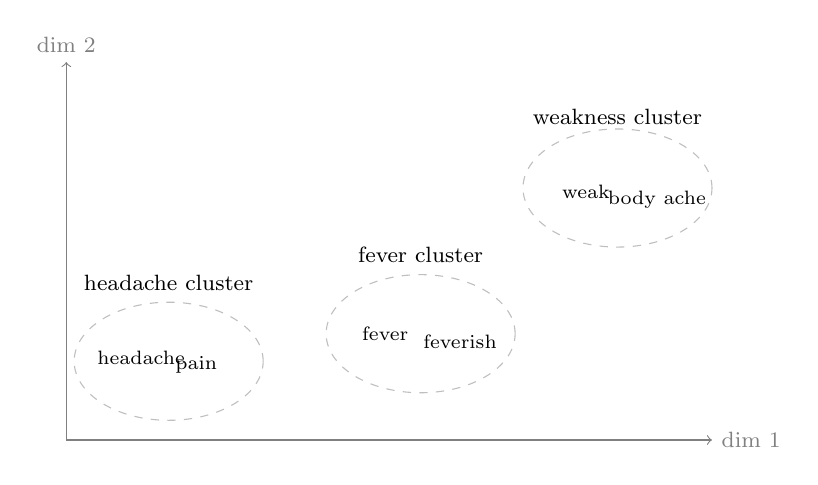
\begin{tikzpicture}[scale=1.0]
  \draw[->, gray] (0,0) -- (8.2,0) node[right, font=\footnotesize] {dim 1};
  \draw[->, gray] (0,0) -- (0,4.8) node[above, font=\footnotesize] {dim 2};
  % Headache cluster
  \draw[dashed, gray!50] (1.3,1.0) ellipse (1.2 and 0.75);
  \node[font=\footnotesize] at (1.3, 2.0) {headache cluster};
  \node[font=\scriptsize] at (0.95, 1.05) {headache};
  \node[font=\scriptsize] at (1.65, 0.95) {pain};
  % Fever cluster
  \draw[dashed, gray!50] (4.5,1.35) ellipse (1.2 and 0.75);
  \node[font=\footnotesize] at (4.5, 2.35) {fever cluster};
  \node[font=\scriptsize] at (4.05, 1.35) {fever};
  \node[font=\scriptsize] at (5.0, 1.25) {feverish};
  % Body / weakness cluster (matches running complaint)
  \draw[dashed, gray!50] (7.0,3.2) ellipse (1.2 and 0.75);
  \node[font=\footnotesize] at (7.0, 4.1) {weakness cluster};
  \node[font=\scriptsize] at (6.6, 3.15) {weak};
  \node[font=\scriptsize] at (7.5, 3.05) {body ache};
\end{tikzpicture}
\caption{Schematic of BioBERT embedding space: familiar symptom words group together after biomedical pre-training (two examples per cluster).}
\label{fig:word-embed}
\end{figure}

When a patient writes ``feverish'' instead of ``fever'', or ``head ache'' as two tokens, the model can still map the wording into regions of this space associated with similar presentations. That generalisation across varied patient language is central to text-first triage.

Contextual mapping sums three embeddings (Equation~\eqref{eq:embedding-sum-preview}). The positional embedding depends only on index \(i\), and the segment embedding depends on segment id \(s\) (always \(s=0\) for a single complaint):
\begin{equation}
  E_{\mathrm{pos}}(i) \in \mathbb{R}^{768}, \qquad E_{\mathrm{seg}}(s) \in \mathbb{R}^{768}, \quad s = 0.
\end{equation}
The final input vector for token \(t_i\) at position \(i\) is the element-wise sum across all \(D=768\) dimensions:
\begin{equation}
  E(t_i)_d = E_{\mathrm{word}}(t_i)_d + E_{\mathrm{pos}}(i)_d + E_{\mathrm{seg}}(s)_d, \quad d = 1, \ldots, 768.
  \label{eq:embedding-sum-full}
\end{equation}
In words: for each dimension \(d\), the word number, the position number, and the segment number are added together. The result is still a single 768-length vector for that token, not three vectors glued end to end.

\subsection{Why three embedding components}

The model does not use a single lookup. Each token must pass through \textbf{three} additive components before the encoder stack, for distinct reasons:
\begin{enumerate}
\item \textbf{Word embedding \(E_{\mathrm{word}}\).} Encodes \emph{what} the subword is (clinical meaning of ``feverish'' versus ``football'').
\item \textbf{Position embedding \(E_{\mathrm{pos}}(i)\).} Encodes \emph{where} the token sits in the complaint. Transformers have no built-in left-to-right recurrence; without position, ``severe pain then mild'' could not be distinguished from the reverse order.
\item \textbf{Segment embedding \(E_{\mathrm{seg}}(s)\).} Marks sentence A versus B in paired BERT tasks. For a single chief complaint we always use \(s=0\); the term is kept so the BioBERT checkpoint remains architecturally compatible even though a second segment is unused at intake.
\end{enumerate}
Omitting word embeddings would remove meaning; omitting position would scramble order-sensitive clinical phrasing; omitting segment would break compatibility with the pre-trained BERT/BioBERT weight layout. The three components are therefore not decorative: they are the minimal input interface the Transformer expects.

\subsection{Why the hidden dimension is \(D = 768\)}

BioBERT-base uses hidden width \(D = 768\). That width is fixed by the published architecture \citep{lee2020biobert,devlin2019bert} and matches
\begin{equation}
  12 \text{ attention heads} \times 64 \text{ dimensions per head} = 768.
\end{equation}
Every token vector, every encoder layer, and the classification summary \(h_{\mathrm{[CLS]}}\) live in \(\mathbb{R}^{768}\). The width is large enough to encode rich biomedical semantics yet small enough to stack twelve layers and train on large corpora. Changing \(D\) would require a different model family; this project therefore keeps \(D=768\) throughout.

\begin{table}[H]
\centering
\small
\begin{tabular}{|l|p{10cm}|}
\hline
\textbf{Symbol} & \textbf{Definition} \\
\hline
\(E_{\mathrm{word}}(t_i)\) & Row of \(E_{\mathrm{word}}\) looked up by token ID \\
\(E_{\mathrm{pos}}(i)\) & Learned vector for position \(i\) in the sequence \\
\(E_{\mathrm{seg}}(s)\) & Learned vector for segment \(s\) (here \(s=0\)) \\
\(E(t_i)_d\) & Component \(d\) of the summed embedding \\
\hline
\end{tabular}
\caption{Symbols in the full input embedding (Equation~\eqref{eq:embedding-sum-full}).}
\label{tab:embed-full-symbols}
\end{table}

\begin{example}
For token ``head'' at position \(i=4\), suppose the first three dimensions (illustrative only) are
\begin{align*}
  E_{\mathrm{word}} &= [0.31,\,-0.18,\,0.52], \\
  E_{\mathrm{pos}}(4) &= [0.05,\,0.02,\,-0.01], \\
  E_{\mathrm{seg}}(0) &= [0.00,\,0.00,\,0.00], \\
  E(t_4) &= E_{\mathrm{word}} + E_{\mathrm{pos}}(4) + E_{\mathrm{seg}}(0) \\
         &= [0.36,\,-0.16,\,0.51] \quad \text{(first three dimensions)}.
\end{align*}
The same element-wise addition repeats for all remaining dimensions \(d=4,\ldots,768\). The result is row 4 of \(H^{(0)}\).
\end{example}

\begin{remark}
The embedding table is like a dictionary: each token ID points to a list of 768 numbers encoding meaning. Adding position tells the model where the word appears; adding segment (zero here) reserves the mechanism for two-sentence inputs in other BERT tasks.
\end{remark}

Figure~\ref{fig:three-embed} shows the flow for one token position. The 768 dimensions are a fixed width chosen in the original BERT architecture: wide enough to encode rich semantics, yet small enough to train twelve layers on large corpora.

\begin{figure}[H]
\centering
\resizebox{0.88\textwidth}{!}{%
\begin{tikzpicture}[node distance=0.6cm and 1.2cm,
  emb/.style={draw=green!60!black, rounded corners, fill=green!8,
    minimum width=2.4cm, minimum height=0.65cm, align=center, font=\small}]
  \node[emb] (ew) {$E_{\mathrm{word}}$\\(token identity)};
  \node[emb, below=of ew] (ep) {$E_{\mathrm{pos}}(i)$\\(position $i$)};
  \node[emb, below=of ep] (es) {$E_{\mathrm{seg}}(0)$\\(segment 0)};
  \node[circle, draw, thick, minimum size=0.7cm, right=2.2cm of ep] (plus) {$+$};
  \node[emb, right=1.2cm of plus] (ef) {$E(t_i)$\\final embedding};
  \node[emb, right=1.2cm of ef, fill=triageYellow!20] (row) {Row $i$ of $H^{(0)}$};
  \draw[flowarr] (ew.east) -| (plus.west);
  \draw[flowarr] (ep) -- (plus);
  \draw[flowarr] (es.east) -| (plus.west);
  \draw[flowarr] (plus) -- (ef);
  \draw[flowarr] (ef) -- (row);
\end{tikzpicture}}
\caption{Three embeddings summed element-wise for one token position.}
\label{fig:three-embed}
\end{figure}

\section{Input matrix \(H^{(0)}\)}
\label{sec:h0}

Stacking the embedding vector for each of the \(M\) tokens forms the initial hidden-state matrix
\begin{equation}
  H^{(0)} \in \mathbb{R}^{M \times 768},
\end{equation}
where \(M \leq 128\) is the padded sequence length and \(768\) is the BioBERT hidden dimension.
\textbf{Rows versus columns.} By convention in this project:
\begin{itemize}
\item \textbf{Rows} (\(M \leq 128\)) index \textbf{token positions} in the sequence (row \(0\) is \texttt{[CLS]}, then the WordPiece tokens, then \texttt{[SEP]} and pads).
\item \textbf{Columns} (\(768\)) index \textbf{hidden feature dimensions} of the BioBERT representation.
\end{itemize}
Row \(i\) is built by applying Equation~\eqref{eq:embedding-sum-full} at position \(i\): look up the word vector, add the positional vector \(E_{\mathrm{pos}}(i)\), add the segment vector \(E_{\mathrm{seg}}(0)\), and stack the result. Viewed this way, a chief complaint is a table of numbers that the encoder layers progressively transform. The same row/column convention holds for \(H^{(\ell)}\) after each encoder layer: shape stays \(M \times 768\); only the entries change as self-attention mixes information \emph{across rows}.

Later, the classification weight matrix \(W \in \mathbb{R}^{5 \times 768}\) uses the complementary layout: \textbf{rows} are the five acuity classes and \textbf{columns} are the \(768\) features that multiply \(h_{\mathrm{[CLS]}}\) (Section~\ref{sec:classification}).

\begin{table}[H]
\centering
\footnotesize
\begin{tabular}{|c|l|c|c|c|c|c|}
\hline
\textbf{\(i\)} & \textbf{Token} & \(D_1\) & \(D_2\) & \(D_3\) & \(D_4\) & \(\cdots\) \\
\hline
0 & \texttt{[CLS]} & \(0.02\) & \(0.11\) & \(-0.05\) & \(0.33\) & \(\cdots\) \\
1 & i & \(-0.08\) & \(0.04\) & \(0.19\) & \(0.01\) & \(\cdots\) \\
2 & have & \(0.15\) & \(-0.22\) & \(0.07\) & \(0.44\) & \(\cdots\) \\
4 & head & \(0.31\) & \(-0.18\) & \(0.52\) & \(0.09\) & \(\cdots\) \\
7 & fever & \(0.44\) & \(0.27\) & \(-0.11\) & \(0.61\) & \(\cdots\) \\
\(\vdots\) & \(\vdots\) & \(\vdots\) & \(\vdots\) & \(\vdots\) & \(\vdots\) & \(\vdots\) \\
\hline
\end{tabular}
\caption{Example submatrix of \(H^{(0)}\) (first four of 768 dimensions; illustrative values).}
\label{tab:submatrix}
\end{table}

After encoding, row 0 (\texttt{[CLS]}) holds the summary passed to the softmax classifier; the remaining rows are not used directly for the final colour decision.

\section{Encoder layers}
\label{sec:encoder}

BioBERT applies the same encoder block \(L=12\) times. Each block first lets tokens attend to one another (mixing symptom phrases), then applies a feed-forward network (FFN) to each row independently. \textbf{Residual connections} add the block input back to its output so that gradients can flow through depth during training. \textbf{Layer normalisation} (\(\mathrm{LayerNorm}\)) rescales each row to zero mean and unit variance for numerical stability \citep{vaswani2017attention,devlin2019bert}. \(\mathrm{MultiHeadAttention}\) is the twelve-head self-attention block of Section~\ref{sec:attention}. \(\mathrm{GELU}\) is the Gaussian Error Linear Unit used in BERT/BioBERT FFNs (smooth nonlinear activation; not ReLU). The update equations are
\begin{align}
  Z^{(\ell)} &= \mathrm{LayerNorm}\!\bigl(H^{(\ell-1)} + \mathrm{MultiHeadAttention}(H^{(\ell-1)})\bigr), \\
  H^{(\ell)} &= \mathrm{LayerNorm}\!\bigl(Z^{(\ell)} + \mathrm{FFN}(Z^{(\ell)})\bigr), \\
  \mathrm{FFN}(x) &= W_2\,\mathrm{GELU}(W_1 x + b_1) + b_2,
\end{align}
where \(H^{(\ell-1)}\) and \(H^{(\ell)}\) are the hidden-state matrices before and after layer \(\ell\), \(Z^{(\ell)}\) is the intermediate state after attention, and \(\mathrm{FFN}\) uses \(W_1 \in \mathbb{R}^{768 \times 3072}\), \(W_2 \in \mathbb{R}^{3072 \times 768}\), and biases \(b_1 \in \mathbb{R}^{3072}\), \(b_2 \in \mathbb{R}^{768}\) in the standard BERT-base configuration. The inner dimension 3072 is four times the hidden width 768, giving the FFN enough capacity to transform each token row nonlinearly. In plain terms, each layer updates every token using the whole complaint, while the residual connection keeps the previous representation so meaning is refined rather than replaced.

\begin{table}[H]
\centering
\small
\begin{tabular}{|p{3.2cm}|p{8.8cm}|}
\hline
\textbf{Component} & \textbf{What it does} \\
\hline
MultiHeadAttention & Twelve parallel self-attention heads; each learns different word relationships \\
FFN & Two linear layers with GELU: expands each row to 3072 dims, then projects back to 768 \\
LayerNorm & Rescales activations for stable training across depth \\
Residual (\(+\)) & Adds sub-layer input to output so earlier information is not lost \\
\hline
\end{tabular}
\caption{Components inside one BioBERT encoder layer.}
\label{tab:encoder-components}
\end{table}

\begin{figure}[H]
\centering
\resizebox{0.45\textwidth}{!}{%
\begin{tikzpicture}[
  node distance=0.35cm and 0.4cm,
  block/.style={draw=green!60!black, rounded corners, fill=green!8,
    minimum width=2.8cm, minimum height=0.55cm, align=center, font=\scriptsize}
]
  \node[block] (in) {Input $H^{(\ell-1)}$};
  \node[block, below=of in] (attn) {Multi-head self-attention};
  \node[block, below=of attn] (add1) {Residual + layer norm $\to Z^{(\ell)}$};
  \node[block, below=of add1] (ffn) {Feed-forward network (FFN)};
  \node[block, below=of ffn] (add2) {Residual + layer norm $\to H^{(\ell)}$};
  \draw[flowarr] (in) -- (attn);
  \draw[flowarr] (attn) -- (add1);
  \draw[flowarr] (add1) -- (ffn);
  \draw[flowarr] (ffn) -- (add2);
  \draw[flowarr, dashed] (in.east) -| ++(1.2,0) |- (add1.east);
  \draw[flowarr, dashed] (add1.east) -| ++(1.2,0) |- (add2.east);
\end{tikzpicture}}
\caption{One BioBERT encoder layer (dashed arrows: residual connections). The block is stacked $L=12$ times.}
\label{fig:encoder-layer}
\end{figure}

In the attention sub-step, each token row is updated using information from every other row in the complaint, which is how ``headache'' and ``feverish'' influence one another before acuity is estimated. The FFN sub-step then applies the same nonlinear transformation to each row separately, increasing representational capacity. Repeating this block twelve times transforms \(H^{(0)}\) into \(H^{(12)}\):
\[
  H^{(0)} \xrightarrow{\text{Layer 1}} H^{(1)} \xrightarrow{\text{Layer 2}} \cdots \xrightarrow{\text{Layer 12}} H^{(12)} = H^{(L)}.
\]
Shallow layers (1--4) tend to encode individual words and short phrases; middle layers (5--8) combine symptoms such as ``headache'' with ``feverish'' and ``weak''; deep layers (9--12) encode broader urgency patterns. All \(M\) token rows are processed in parallel at each layer, not left-to-right as in older language models.

\begin{remark}
Stacking layers is like reading a complaint once for words, once for symptom combinations, and once for overall urgency. The \texttt{[CLS]} row at layer 12 becomes \(h_{\mathrm{[CLS]}}\) for classification.
\end{remark}

\section{Self-attention}
\label{sec:attention}

Self-attention computes a weighted combination of token representations for each position. The computation proceeds in four steps, matching Figure~\ref{fig:self-attention}:

\begin{enumerate}
\item \textbf{Project} hidden rows into query, key, and value matrices.
\item \textbf{Score} pairwise compatibility between tokens.
\item \textbf{Normalise} scores into attention weights.
\item \textbf{Combine} value rows into context-aware outputs.
\end{enumerate}
Let \(H = H^{(\ell-1)} \in \mathbb{R}^{M \times 768}\) be the input to the current encoder layer. Learned projection matrices \(W_Q, W_K, W_V \in \mathbb{R}^{768 \times d_k}\) with key dimension \(d_k = 64\) produce
\begin{align*}
  Q &= H W_Q, \quad K = H W_K, \quad V = H W_V, \\
  S &= QK^\top / \sqrt{d_k}, \\
  A &= \mathrm{softmax}(S), \\
  \text{output} &= AV,
\end{align*}
where \(Q,K,V \in \mathbb{R}^{M \times d_k}\), \(S\) and \(A\) are \(M \times M\) score and weight matrices, and \(\mathrm{softmax}\) is applied row-wise so each query distributes weights that sum to~1.

Following \citet{vaswani2017attention}, one attention head uses:
\begin{equation}
  \mathrm{Attention}(Q,K,V) = \mathrm{softmax}\!\left(\frac{QK^{\top}}{\sqrt{d_k}}\right)V,
  \label{eq:attention}
\end{equation}
with key dimension \(d_k = 64\) per head. For one query row, the softmax over keys assigns weight \(\alpha_j\) to token \(j\):
\begin{equation}
  \alpha_j = \frac{\exp(e_j)}{\sum_{k=1}^{M}\exp(e_k)}, \quad \sum_{j=1}^{M}\alpha_j = 1,
  \label{eq:attn-softmax}
\end{equation}
where \(e_j\) is the scaled score in row \(j\) of \(QK^\top/\sqrt{d_k}\) and \(M\) is the sequence length (at most 128). BioBERT runs twelve such heads in parallel; their outputs are concatenated and projected back to 768 dimensions so each head can specialise (e.g.\ symptom co-occurrence vs negation).

\begin{remark}
In triage language: \(Q\) is what the current token looks for in the rest of the complaint; \(K\) is the label each other token shows; \(V\) is the meaning that is mixed in when the match is strong. Dividing by \(\sqrt{d_k}\) keeps the match scores from becoming too large before Softmax. The Softmax inside Equation~\eqref{eq:attention} only mixes \textbf{token} meanings; it is not the five-class Softmax that later chooses the colour.
\end{remark}

\begin{figure}[H]
\centering
\resizebox{0.75\textwidth}{!}{%
\begin{tikzpicture}[node distance=0.7cm, thick,
  box/.style={draw=green!60!black, rectangle, fill=green!5, text width=3.2cm, align=center, minimum height=0.75cm, rounded corners, font=\small},
  highlightbox/.style={draw=green!80!black, rectangle, fill=green!20, text width=4.2cm, align=center, minimum height=0.7cm, rounded corners, font=\small\bfseries},
  arrow/.style={->, >=latex, thick, draw=black!70},
  label/.style={font=\tiny\itshape, text=black!70, align=center}]
  \node[highlightbox] (input) {1.\ Input Embeddings\\ \mdseries \footnotesize (token rows of $H^{(\ell-1)}$)};
  \node[box, below=0.7cm of input, xshift=-3.8cm] (query) {\textbf{Query ($Q$)}\\ \footnotesize ``What am I looking for?''};
  \node[box, below=0.7cm of input] (key) {\textbf{Key ($K$)}\\ \footnotesize ``What do I represent?''};
  \node[box, below=0.7cm of input, xshift=3.8cm] (value) {\textbf{Value ($V$)}\\ \footnotesize ``What is my content?''};
  \node[box, fill=yellow!20, draw=yellow!80!black, below=0.7cm of key, text width=4cm] (matmul) {\textbf{2.\ Alignment Scores}\\ $Q \cdot K^T$};
  \node[box, fill=orange!20, draw=orange!80!black, below=0.7cm of matmul, text width=4cm] (softmax) {\textbf{3.\ Softmax Normalization}};
  \node[highlightbox, fill=red!15, draw=red!80!black, below=0.7cm of softmax, text width=4.2cm] (output) {\textbf{4.\ Context-Aware Output}\\ \mdseries \footnotesize Weighted sum ($Attention \times V$)};
  \draw[arrow] (input) -- node[label, left] {Linear\\Transform} (query);
  \draw[arrow] (input) -- node[label, right] {Linear\\Transform} (key);
  \draw[arrow] (input) -- node[label, right] {Linear\\Transform} (value);
  \draw[arrow] (query) |- (matmul);
  \draw[arrow] (key) -- (matmul);
  \draw[arrow] (matmul) -- node[label, right] {Scale by $\frac{1}{\sqrt{d_k}}$} (softmax);
  \draw[arrow] (softmax) -- (output);
  \draw[arrow] (value) |- (output);
\end{tikzpicture}}
\caption{Self-attention data flow within one encoder layer (schematic architecture diagram; not extracted model weights).}
\label{fig:self-attention}
\end{figure}

\begin{table}[H]
\centering
\small
\begin{tabular}{|l|p{10cm}|}
\hline
\textbf{Symbol} & \textbf{Definition} \\
\hline
\(H = H^{(\ell-1)}\) & Hidden-state matrix entering the current encoder layer (\(M \times 768\)) \\
\(W_Q, W_K, W_V\) & Learned projection matrices (\(768 \times d_k\)) that form queries, keys, and values \\
\(Q, K, V\) & Query, key, and value matrices (\(M \times d_k\)) derived from \(H\) \\
\(QK^\top\) & Matrix of pairwise compatibility scores between tokens \\
\(\sqrt{d_k}\) & Scaling constant (\(d_k=64\)) that prevents dot products from growing too large \\
\(e_j\) & Raw attention score for token \(j\) before normalisation \\
\(\alpha_j\) & Normalised attention weight for token \(j\) (a probability) \\
\(M\) & Sequence length (number of tokens, at most 128) \\
\hline
\end{tabular}
\caption{Self-attention notation.}
\label{tab:attention-symbols}
\end{table}

\begin{table}[H]
\centering
\small
\begin{tabular}{|l|c|c|c|c|}
\hline
Query token & \texttt{[CLS]} & headache & feverish & filler \\
\hline
Attention to & 0.09 & 0.32 & 0.41 & 0.18 \\
\hline
\end{tabular}
\caption{Schematic attention weights when the query is \texttt{[CLS]} (illustrative, not measured from the model). Symptom tokens receive higher weight than filler words.}
\label{tab:attn-toy}
\end{table}

The product \(QK^\top\) measures how strongly each token should attend to every other token. Dividing by \(\sqrt{d_k}\) keeps those scores in a range where the softmax in Equation~\eqref{eq:attn-softmax} does not saturate. In a complaint mentioning both ``headache'' and ``feverish'', attention typically assigns higher weight to symptom tokens than to function words such as ``I'' or ``and'', so the updated representation emphasises clinically informative wording (Table~\ref{tab:attn-toy}).

\section{Classification softmax}
\label{sec:classification}

\subsection{Mutually exclusive acuity categories}

When a patient submits a chief complaint, their clinical urgency for routing is treated as falling into \textbf{exactly one} of the five SATS-aligned acuity levels \(\{1,2,3,4,5\}\). A presentation cannot be Level~1 (immediate) and Level~5 (routine) at the same decision instant. Because only one level is selected for the pathway colour, the five categories are modelled as \textbf{mutually exclusive}. That modelling choice determines the output layer: the network must produce a distribution over five options, not five independent yes/no scores.

If the head used five independent sigmoid units, each class probability could be high at once (for example \(\hat{y}_1=0.9\) and \(\hat{y}_5=0.8\)), which would not define a single routing colour. Softmax avoids that inconsistency by normalising across the five logits together.

\subsection{Softmax as the probability translator}

After BioBERT encoding, the classification head maps the summary vector \(h_{\mathrm{[CLS]}} \in \mathbb{R}^{768}\) to five unconstrained real scores called \textbf{logits}:
\begin{equation}
\begin{aligned}
  \mathbf{z} &= W h_{\mathrm{[CLS]}} + \mathbf{b}, \\
  \hat{\mathbf{y}} &= \mathrm{softmax}(\mathbf{z}), \\
  \hat{y}_c &= \frac{\exp(z_c)}{\sum_{j=1}^{5}\exp(z_j)},
\end{aligned}
  \label{eq:softmax-class}
\end{equation}
with \(W \in \mathbb{R}^{5 \times 768}\) (\textbf{rows} = acuity classes, \textbf{columns} = features), \(\mathbf{b} \in \mathbb{R}^{5}\), logits \(z_c\), and \(\sum_{c=1}^{5} \hat{y}_c = 1\). Softmax enforces the two elementary rules of a finite probability distribution: every \(\hat{y}_c\) is non-negative, and the five values sum to one. The predicted level is \(\hat{c} = \arg\max_c \hat{y}_c\). Expressing output as probabilities allows downstream routing logic to consider confidence (for example a dominant Yellow at about \(69\%\) versus a near tie between Yellow and Green).

\begin{remark}
The vector \(\mathbf{z}\) holds five \textbf{raw scores (logits)}, not probabilities: a larger \(z_c\) only means that urgency level looks stronger. Softmax turns those scores into five chances that add to~1. The largest chance is the acuity level used for the SATS colour.
\end{remark}

This \textbf{classification Softmax} (over five acuity classes) is distinct from the \textbf{attention Softmax} inside each encoder layer (over token positions). Both use the same functional form; they act on different axes of the model. Attention Softmax asks ``which tokens matter for this query?''; classification Softmax asks ``which acuity level is most probable for this complaint?''

\begin{remark}
The linear map \(\mathbf{z}=W h_{\mathrm{[CLS]}}+\mathbf{b}\) is the triage analogue of a multi-class ``score sheet'': each row of \(W\) emphasises features in \(h_{\mathrm{[CLS]}}\) that favour one acuity level. Softmax then converts those raw scores into a comparable probability vector for hospital routing.
\end{remark}

\subsection{Categorical distribution (\(K=5\))}

By producing five probabilities that sum to one, Softmax parameterises a \textbf{Categorical distribution} over the acuity levels. A Categorical distribution is the discrete law for exactly \(K\) mutually exclusive outcomes; here \(K=5\). The vector \(\hat{\mathbf{y}}\) is the parameter of that law:
\begin{equation}
  \hat{y}_c = P(\text{acuity}=c \mid X), \qquad c\in\{1,2,3,4,5\},
\end{equation}
where \(X\) is the chief complaint and \(\hat{y}_c\) is the Softmax probability of acuity level \(c\).
Informally, \(\hat{\mathbf{y}}\) behaves like a weighted five-sided die whose face probabilities are determined by the complaint text. Sampling from that die would draw a random acuity; hospital routing instead takes the mode \(\hat{c}=\arg\max_c\hat{y}_c\) (and may escalate to a nurse when the mode is not dominant).

Stage~3 training maximises the probability of the ESI-style label under this Categorical model. Equivalently, it minimises the negative log-likelihood (NLL)
\begin{equation}
  \mathcal{L}_{\mathrm{NLL}} = -\log \hat{y}_{y} = -\log P(y\mid X),
\end{equation}
where \(y\) is the true acuity label, \(X\) is the complaint, and \(\hat{y}_{y}=P(y\mid X)\) is the Softmax probability of that label. This is exactly the cross-entropy loss used in Section~\ref{sec:training-pipeline} when labels are one-hot.

\subsection{Bernoulli as the \(K=2\) building block}

The \textbf{Bernoulli} distribution is the two-outcome special case (\(K=2\)): a single trial with results \(\{0,1\}\) and success probability \(p\). Softmax with two logits \((z_0,z_1)\) yields
\begin{equation}
  p = \frac{\exp(z_1)}{\exp(z_0)+\exp(z_1)} = \sigma(z_1-z_0),
\end{equation}
where \(z_0\) and \(z_1\) are the two class logits, \(p\) is the probability of class~1, and \(\sigma(u)=1/(1+e^{-u})\) is the logistic sigmoid. That identity shows why binary logistic regression is Softmax with \(K=2\). The five-class triage head is the same mathematical idea generalised from a weighted coin to five mutually exclusive faces.

\begin{example}[Bernoulli building block]
Suppose a toy two-class head distinguishes ``urgent'' versus ``non-urgent'' with logits \(z_{\mathrm{U}}=1.0\) and \(z_{\mathrm{N}}=-0.5\). Then
\begin{align*}
  \exp(z_{\mathrm{U}}) &= e^{1.0}\approx 2.72, \\
  \exp(z_{\mathrm{N}}) &= e^{-0.5}\approx 0.61, \\
  P(\mathrm{urgent}) &= \frac{2.72}{2.72+0.61}\approx 0.82.
\end{align*}
Raising \(z_{\mathrm{U}}\) relative to \(z_{\mathrm{N}}\) increases urgent probability exactly as raising one acuity logit relative to the others increases that class probability in the five-class Softmax.
\end{example}

\begin{table}[H]
\centering
\small
\begin{tabular}{|l|p{10cm}|}
\hline
\textbf{Symbol} & \textbf{Definition} \\
\hline
\(h_{\mathrm{[CLS]}}\) & 768-dimensional summary vector from final encoder layer \\
\(W, \mathbf{b}\) & Learned classification weight matrix (\(5\times 768\)) and bias \\
\(z_c\) & Logit (pre-softmax score) for acuity level \(c\) \\
\(\hat{y}_c\) & Categorical probability of level \(c \in \{1,\ldots,5\}\) \\
\(\hat{c}\) & Predicted level: index of largest \(\hat{y}_c\) \\
\hline
\end{tabular}
\caption{Classification head notation.}
\label{tab:class-symbols}
\end{table}

\begin{example}[Five-class Softmax for the running complaint]
Suppose illustrative logits for levels 1--5 are
\begin{align*}
  \mathbf{z} &= [-1.2,\,-0.5,\,1.8,\,0.3,\,-0.9], \\
  \exp(\mathbf{z}) &\propto [0.30,\,0.61,\,6.05,\,1.35,\,0.41], \\
  \sum_{c=1}^{5} \exp(z_c) &= 8.72, \\
  \hat{\mathbf{y}} &\approx [0.03,\,0.07,\,0.69,\,0.15,\,0.05], \\
  \hat{c} &= 3, \\
  f_{\mathrm{SATS}}(3) &= \text{Yellow}.
\end{align*}
Level 3 has the largest Categorical probability (\(\hat{y}_3 \approx 0.69\), rounded to 72\% in some deployment logs; Section~\ref{sec:fsats}). The mass on neighbouring Orange (\(0.07\)) and Green (\(0.15+0.05\)) shows residual uncertainty: Softmax does not claim certainty, only a ranked distribution suitable for pathway assist with nurse oversight when confidence is low.
\end{example}

\begin{remark}
Softmax probabilities are calibrated only to the extent that the training distribution matches live intake. High \(\hat{y}_c\) on Triagegeist validation text is not a clinical guarantee at \examplehospital{}; low-confidence or contradictory presentations remain mandatory nurse review.
\end{remark}

\section{Model training pipeline}
\label{sec:training-pipeline}

The deployed triage classifier is not trained from random initialisation. It is the product of three sequential stages: biomedical pre-training (Stage 1), encoder transfer from a prior triage checkpoint (Stage 2), and project fine-tuning on synthetic Triagegeist chief-complaint / ESI-style label pairs (Stage 3). Stages 1 and 2 supply medical language and partial triage adaptation; Stage 3 is the comprehensive retraining that maps free-text complaints to five acuity levels for this chatbot.

\begin{figure}[H]
\centering
\resizebox{0.92\textwidth}{!}{%
\begin{tikzpicture}[
  node distance=0.45cm and 0.35cm,
  stage/.style={draw=green!60!black, rounded corners, fill=green!8,
    minimum width=2.6cm, minimum height=0.85cm, align=center, font=\scriptsize},
  arrow/.style={->, >=latex, thick, draw=black!60}]
  \node[stage] (s1) {Stage 1\\BioBERT MLM\\PubMed + PMC};
  \node[stage, right=of s1] (s2) {Stage 2\\Encoder transfer\\2-class checkpoint};
  \node[stage, right=of s2] (s3) {Stage 3\\Project fine-tuning\\80k complaints, 5 classes};
  \node[stage, right=of s3, fill=triageYellow!25] (out) {Deployed\\triage model};
  \foreach \a/\b in {s1/s2, s2/s3, s3/out} \draw[arrow] (\a) -- (\b);
\end{tikzpicture}}
\caption{Three-stage training stack for the BioBERT triage classifier.}
\label{fig:training-stages}
\end{figure}

\subsection{Stage 1: BioBERT pre-training (masked language modelling)}
\label{sec:mlm}

Before any triage labels are used, BioBERT is trained on biomedical text with masked language modelling (MLM). Random tokens are hidden and the model must predict them from surrounding context in both directions:
\begin{equation}
  \mathcal{L}_{\mathrm{LM}} = -\sum_{i \in \mathcal{M}} \log P(t_i \mid H^{(L)};\, \theta),
\end{equation}
where \(\mathcal{M}\) is the set of masked positions, \(t_i\) is the true token at position \(i\), \(H^{(L)}\) is the final hidden-state matrix from all twelve layers, \(\theta\) denotes all model parameters, and \(P(t_i \mid \cdot)\) is the softmax probability assigned to the correct word. PubMed abstracts and PubMed Central full text (\(\approx 18\) billion words) teach medical vocabulary and syntax. Stage 1 does \textbf{not} teach triage urgency, SATS colours, or informal chief-complaint phrasing.

\begin{table}[H]
\centering
\small
\begin{tabular}{|l|p{10cm}|}
\hline
\textbf{Symbol} & \textbf{Definition} \\
\hline
\(\mathcal{M}\) & Set of masked token positions in the sentence \\
\(t_i\) & True (correct) word at masked position \(i\) \\
\(\theta\) & All model weights and biases \\
\(P(t_i \mid H^{(L)};\,\theta)\) & Model probability for the correct token \\
\(\mathcal{L}_{\mathrm{LM}}\) & Total MLM penalty; lower means better predictions \\
\hline
\end{tabular}
\caption{Masked language modelling notation (Stage 1).}
\label{tab:mlm-symbols}
\end{table}

\begin{example}
If the masked token should be ``headache'', the MLM contribution is
\begin{align*}
  \shortintertext{Good prediction (\(P = 0.92\)):}
  -\log(0.92) &\approx 0.08 && \text{(small penalty)}, \\
  \shortintertext{Poor prediction (\(P = 0.01\)):}
  -\log(0.01) &\approx 4.6 && \text{(large penalty)}.
\end{align*}
\end{example}

\subsection{Stage 2: Encoder transfer from a triage checkpoint}

A publicly available BioBERT triage checkpoint partially adapted the encoder to urgency-related text using a \textbf{two-class} classification head (\(W \in \mathbb{R}^{2 \times 768}\)). For this project, that 2-class head is \textbf{discarded} on load because our labels require five acuity levels. The loader uses \texttt{ignore\_mismatched\_sizes=True}: only encoder weights carry forward; the output layer is randomly reinitialised for five classes. Stage 2 therefore contributes triage-oriented encoder features without constraining the final colour mapping.

\subsection{Stage 3: Fine-tuning on synthetic Triagegeist chief-complaint / ESI-style label pairs}
\label{sec:training}

Stage 3 is the comprehensive retraining performed for this project. ESI-style acuity labels from the synthetic Triagegeist benchmark (Section~\ref{sec:data-provenance}) are inner-joined with chief-complaint text on patient identifier, yielding \(N = 80{,}000\) English text-label pairs \((X_i, y_i)\). Only the free-text English chief complaint (why the patient came) and the ESI-style urgency label (\(1\)--\(5\)) are used; vitals and demographics in the source records are excluded so the NLP path matches the single-shot text input at intake.

The data are split 90/10 into training and validation sets (\(\approx 72{,}000\) / \(\approx 8{,}000\) rows, \texttt{test\_size=0.1}, random seed 42). A new classification head \(W \in \mathbb{R}^{5 \times 768}\), \(\mathbf{b} \in \mathbb{R}^{5}\) is trained from scratch while encoder weights are updated with a small learning rate.

\begin{table}[H]
\centering
\small
\begin{tabular}{|l|r|r|l|}
\hline
\textbf{Level} & \textbf{Count} & \textbf{Proportion} & \textbf{SATS colour} \\
\hline
1 (most urgent) & 3,222 & 0.0403 & Red \\
2 & 13,439 & 0.1680 & Orange \\
3 & 28,921 & 0.3615 & Yellow \\
4 & 23,020 & 0.2878 & Green \\
5 (least urgent) & 11,398 & 0.1425 & Green \\
\hline
\textbf{Total} & \textbf{80,000} & \textbf{1.000} & \\
\hline
\end{tabular}
\caption{Class distribution in the 80{,}000 labeled chief-complaint training pairs.}
\label{tab:class-distribution}
\end{table}

\begin{table}[H]
\centering
\small
\begin{tabular}{|l|l|}
\hline
\textbf{Hyperparameter} & \textbf{Value} \\
\hline
Epochs & 3 \\
Batch size (train and eval) & 16 \\
Learning rate \(\alpha\) & \(2 \times 10^{-5}\) \\
Weight decay & 0.01 \\
Max sequence length & 128 tokens \\
Mixed precision (FP16) & Enabled \\
Total optimizer steps & 13,500 (3 epochs \(\times\) 4,500 steps) \\
Best validation loss & 0.001812 (epoch 3) \\
\hline
\end{tabular}
\caption{Fine-tuning hyperparameters (Stage 3).}
\label{tab:hyperparams}
\end{table}

\begin{table}[H]
\centering
\small
\begin{tabular}{|l|p{8.5cm}|}
\hline
\textbf{Component} & \textbf{Updated during Stage 3?} \\
\hline
Embedding layers & Yes (small learning-rate updates) \\
12 transformer encoder layers & Yes \\
Classification head \(W, \mathbf{b}\) & Yes (trained from scratch) \\
\hline
\end{tabular}
\caption{Which model components change during project fine-tuning.}
\label{tab:trainable-components}
\end{table}

The objective is \textbf{cross-entropy loss}: for each training example, the model is penalised when it assigns low probability to the nurse's true acuity label. For a single example with true class \(y\),
\begin{equation}
  \mathcal{L}_{\mathrm{CE}} = -\log \hat{y}_{y},
\end{equation}
where \(y \in \{1,\ldots,5\}\) is the ESI-style acuity label and \(\hat{y}_{y}\) is the Softmax probability the model assigns to that correct level. Over the full training set the same symbol denotes the empirical risk
\begin{equation}
  \mathcal{L}_{\mathrm{CE}} = -\sum_{i=1}^{N} \log P(y_i \mid X_i;\, \theta), \quad N = 80{,}000,
\end{equation}
where \(X_i\) is complaint \(i\), \(y_i\) is its label, \(\theta\) denotes all trainable parameters, and \(P(y_i \mid X_i;\, \theta)=\hat{y}_{y_i}\) is the predicted probability of the true class.

\begin{example}
If the nurse labeled a complaint Yellow (level 3), the cross-entropy penalty is
\begin{align*}
  \shortintertext{Low confidence on the true class (\(\hat{y}_3 = 0.05\)):}
  \mathcal{L}_{\mathrm{CE}} = -\log(0.05) &\approx 3.0 && \text{(large penalty)}, \\
  \shortintertext{High confidence on the true class (\(\hat{y}_3 = 0.95\)):}
  \mathcal{L}_{\mathrm{CE}} = -\log(0.95) &\approx 0.05 && \text{(small penalty)}.
\end{align*}
Fine-tuning adjusts weights so correct classes receive higher probability on similar complaints.
\end{example}

\textbf{Backpropagation} computes how each weight contributed to \(\mathcal{L}_{\mathrm{CE}}\) by applying the chain rule backward from the loss through the softmax head and all twelve encoder layers. For classification weights \(W \in \mathbb{R}^{5 \times 768}\), with logits \(\mathbf{z} = W h_{\mathrm{[CLS]}} + \mathbf{b}\) where \(h_{\mathrm{[CLS]}} \in \mathbb{R}^{768}\) is the final summary vector and \(\mathbf{b} \in \mathbb{R}^{5}\) is the bias,
\begin{equation}
  \frac{\partial \mathcal{L}_{\mathrm{CE}}}{\partial W} = \frac{\partial \mathcal{L}_{\mathrm{CE}}}{\partial \hat{\mathbf{y}}} \cdot \frac{\partial \hat{\mathbf{y}}}{\partial \mathbf{z}} \cdot \frac{\partial \mathbf{z}}{\partial W}.
\end{equation}
In words: (i) \(\partial \mathcal{L}_{\mathrm{CE}}/\partial \hat{\mathbf{y}}\) measures how wrong the predicted probabilities are; (ii) \(\partial \hat{\mathbf{y}}/\partial \mathbf{z}\) propagates through softmax; (iii) \(\partial \mathbf{z}/\partial W\) links logits to the weight matrix. The same logic applies layer by layer through BioBERT.

\textbf{Gradient descent} then adjusts weights in the direction that reduces the loss:
\begin{equation}
  W_{\mathrm{new}} = W_{\mathrm{old}} - \alpha \frac{\partial \mathcal{L}_{\mathrm{CE}}}{\partial W},
\end{equation}
where \(\alpha = 2 \times 10^{-5}\) is the learning rate, \(W_{\mathrm{old}}\) is the current weight matrix, and \(W_{\mathrm{new}}\) is the updated matrix. When the model confidently predicts the wrong colour, backpropagation increases the loss sharply and the subsequent weight update pushes similar complaints toward the ESI-style class on the next training pass.

\begin{remark}
Pre-training (Stage 1) gives the model medical language; comprehensive fine-tuning (Stage 3) teaches triage decisions on short, informal chief-complaint phrasing. The learning rate is kept small so PubMed knowledge is preserved while the head and encoder adapt to urgency labels.
\end{remark}

\subsection{Mitigating class imbalance}
\label{sec:imbalance-mitigation}

Table~\ref{tab:class-distribution} shows that Level~3 dominates Triagegeist while Level~1 (Red) is scarce. The published \emph{stratified-oversampling} checkpoint therefore rebalances the \textbf{training} split only (the validation split is left untouched) before a second Stage~3 run, with embedding-space SMOTE disabled (\texttt{USE\_EMBEDDING\_SMOTE=False}). The algorithmic steps are:

\begin{enumerate}
\item Restrict imbalance mitigation to the stratified Triagegeist training rows from Section~\ref{sec:training}.
\item Apply light \textbf{text augmentation} to minority urgent classes (acuity levels \(1\) and \(2\)): synonym or paraphrase variants of the chief-complaint string, with protected medical keywords left unchanged. Configured yields are two augmented variants per Level~1 row and one per Level~2 row.
\item Apply \textbf{random minority oversampling} with replacement until target counts \(n_1 = 10{,}000\) and \(n_2 = 15{,}000\); Levels~$3$--$5$ keep their natural training counts.
\item Run end-to-end Stage~3 fine-tuning (WordPiece \(\rightarrow\) BioBERT \(\rightarrow\) Softmax) on the expanded training set with the same hyperparameters as Table~\ref{tab:hyperparams}.
\end{enumerate}

Chapter~\ref{ch:results} contrasts this checkpoint with the unrebalanced baseline and explains why classical embedding SMOTE was not chosen (Section~\ref{sec:oversampling-choice}).

\section{Mapping acuity to colour: \(f_{\mathrm{SATS}}\)}
\label{sec:fsats}

\subsection{ESI-to-SATS mapping assumption}

The Softmax head predicts Emergency Severity Index (ESI)--style acuity levels \(1\)--\(5\) learned from synthetic Triagegeist training pairs and scored on external MIMIC-IV-ED and NHAMCS labels. Those sources are \textbf{not} SATS-labelled: ESI is primarily resource-based, whereas SATS combines vital-sign TEWS with clinical discriminators. No direct SATS colour labels are used for training. Hospital routing at \examplehospital{} nonetheless uses SATS colours, so this project defines a fixed deterministic operational heuristic \(f_{\mathrm{SATS}}\) that converts an ESI-style level into a SATS-aligned colour for text-first routing assist:
\begin{equation}
  f_{\mathrm{SATS}}(\hat{c}) = C_{\mathrm{NLP}} = \begin{cases}
    \text{Red} & \hat{c} = 1 \\
    \text{Orange} & \hat{c} = 2 \\
    \text{Yellow} & \hat{c} = 3 \\
    \text{Green} & \hat{c} \in \{4, 5\}
  \end{cases}
\end{equation}
where \(\hat{c} = \arg\max_c \hat{y}_c\) is the predicted acuity level, \(f_{\mathrm{SATS}}\) is the fixed level-to-colour map, and \(C_{\mathrm{NLP}}\) is the resulting SATS-aligned colour from the text path.

Both systems contain five ordered urgency categories, allowing the construction of an ordinal heuristic mapping for this prototype. This structural similarity does \emph{not} imply clinical equivalence. The map \(f_{\mathrm{SATS}}\) is a proposed operational crosswalk for intake assistance, not a validated clinical translation, and requires adjudication against clinician-assigned SATS colours before operational claims beyond routing assist.

\begin{table}[H]
\centering
\small
\begin{tabular}{|c|l|l|}
\hline
\textbf{ESI-style level} & \textbf{Clinical name} & \(f_{\mathrm{SATS}}(\ell)\) \\
\hline
1 & Resuscitation & Red \\
2 & Emergent & Orange \\
3 & Urgent & Yellow \\
4 & Less urgent & Green \\
5 & Non-urgent & Green \\
\hline
\end{tabular}
\caption{Proposed ESI-style acuity \(\rightarrow\) SATS colour heuristic for text-first routing (not a clinical equivalence table).}
\label{tab:fsats-esi}
\end{table}

Levels 4 and 5 both map to Green because both are non-urgent in the five-level schema. Blue is reserved for dignity protocol on arrival and is not produced by this five-class head. Colour accuracy is therefore not equivalent to five-class accuracy: \(f_{\mathrm{SATS}}\) is many-to-one on \(\{4,5\}\).

\section{Clinical pathways \(P(C_{\mathrm{NLP}})\)}
\label{sec:pathways}

Once \(C_{\mathrm{NLP}}\) is known, the chatbot attaches a pathway card that specifies waiting time, destination, and escalation rules drawn from SATS-aligned hospital protocol at \examplehospital{}:
\begin{equation}
  P(C_{\mathrm{NLP}}) = \bigl(T_{\max},\; \text{destination},\; \text{actions},\; \text{escalation}\bigr),
\end{equation}
where \(P(C_{\mathrm{NLP}})\) is the pathway card for colour \(C_{\mathrm{NLP}}\), \(T_{\max}\) is the maximum waiting time, destination is the primary clinical department, actions list support steps (nursing, pharmacy, diagnostics), and escalation defines what happens if the timer expires or the patient worsens. Colour alone is not enough at intake: the pathway card names where the patient should go and how soon they should be seen. The four tuple components correspond directly to the columns in Table~\ref{tab:pathways}.

\textbf{Age-agnostic classifier.} The current classifier maps \(X\to\hat{y}\), not \((X,\mathrm{age})\to\hat{y}\). BioBERT has no age feature, so Pediatrics is never a default destination for adult ASTS colours and paediatric TEWS tables remain out of scope. Before the pathway card is finalised, a deterministic (non-neural) check runs on the complaint \(X\). Define the marker set
\begin{equation}
  \mathcal{M}_{\mathrm{child}}=\{\texttt{child},\,\texttt{son},\,\texttt{daughter},\,\texttt{baby},\,\texttt{infant},\,\texttt{toddler}\}.
\end{equation}
Normalise \(X\) to lowercase. If any element of \(\mathcal{M}_{\mathrm{child}}\) appears as a substring of \(X\), override the destination field of \(P(C_{\mathrm{NLP}})\) to Pediatrics; otherwise keep the adult destination for that colour. This rule is applied after \(C_{\mathrm{NLP}}=f_{\mathrm{SATS}}(\hat{c})\) and does not change the colour itself.

The pathway configuration below represents the authors' documented interpretation of observed workflow at \examplehospital{} and published SATS rules; it should not be interpreted as an official clinical protocol unless formally approved by the hospital.

\begin{table}[H]
\centering
\small
\begin{tabular}{|l|l|p{3.2cm}|p{3.5cm}|}
\hline
\textbf{Colour} & \(T_{\max}\) & \textbf{Destination} & \textbf{Escalation} \\
\hline
Red & 0 min & Resuscitation / Surgery & Immediate senior alert \\
Orange & 10 min & Internal Medicine / Surgery / Obs.\ \& Gynae & Head nurse if unclaimed \\
Yellow & 60 min & Outpatient urgent stream & Re-assess if timer expires \\
Green & \(<\) 4 h & Outpatient / Dental / Eye / Public \& Preventive Health & Return only if worse \\
\hline
\end{tabular}
\caption{SATS pathway protocol at \examplehospital{} (clinical destinations; adult ASTS default).}
\label{tab:pathways}
\end{table}

Table~\ref{tab:pathway-scenarios} is the authoritative full map: one row per NLP outcome (including gate rejection), with primary clinical departments, support actions, escalation rules, and an example complaint phrase.

\begin{table}[H]
\centering
\scriptsize
\begin{tabular}{|p{1.5cm}|p{1.6cm}|p{0.9cm}|p{2.4cm}|p{3.1cm}|p{2.2cm}|}
\hline
\textbf{Scenario} & \textbf{Trigger} & \(T_{\max}\) & \textbf{Primary clinical departments} & \textbf{Support actions} & \textbf{Escalation} \\
\hline
Gate reject & \(g(X)<0.30\) & n/a & Hold at intake & Nursing: request complaint; HIT: no colour stored & Re-submit with clinical text \\
Red & \(\hat{c}=1\) & 0 min & Surgery, Internal Medicine & Nursing (vitals, TEWS), Pharmacy (emergency), Health Info (Red flag), Admin (bed bypass), HIT (Code Red) & Immediate senior clinician \\
Orange & \(\hat{c}=2\) & 10 min & Internal Medicine, Surgery, Obs.\ \& Gynae & Nursing (monitor, timer), Diagnostics (stat labs), Pharmacy, Health Info, Admin, HIT & Head nurse if unclaimed \\
Yellow & \(\hat{c}=3\) & 60 min & Outpatient urgent, Diagnostics & Nursing (vitals, TEWS, timer), Pharmacy, Health Info, HIT, Accounts (defer billing) & Re-assess at 60 min \\
Green & \(\hat{c}\in\{4,5\}\) & \(<\)4 h & Outpatient, Dental, Eye, Public \& Preventive Health & Nursing (brief triage), Diagnostics (routine), Health Info, HIT, Accounts & Return if worse \\
\hline
\end{tabular}
\caption{Complete NLP pathway scenarios at \examplehospital{} (gate reject plus four SATS colours). Pediatrics is not a default Yellow destination; destination is overridden to Pediatrics only when the lexical child-marker rule matches \(\mathcal{M}_{\mathrm{child}}\) in \(X\).}
\label{tab:pathway-scenarios}
\end{table}

\begin{table}[H]
\centering
\scriptsize
\begin{tabular}{|l|p{10cm}|}
\hline
\textbf{Scenario} & \textbf{Example complaint phrase} \\
\hline
Gate reject & ``Hello, how are you?'' (no clinical content) \\
Red & ``Crushing chest pain, cannot breathe, sweating heavily'' \\
Orange & ``Severe abdominal pain in pregnancy, bleeding'' \\
Yellow & \runningcomplaint{} \\
Green & ``Routine dental pain for two weeks, no fever'' \\
\hline
\end{tabular}
\caption{Example chief complaints triggering each pathway scenario.}
\label{tab:pathway-examples}
\end{table}

Table~\ref{tab:knust-dept-routing} maps all hospital departments to their role in the pathway system. Clinical departments receive patients by colour; support departments execute actions attached to each pathway card.

\begin{table}[H]
\centering
\scriptsize
\begin{tabular}{|p{3.4cm}|c|p{4.8cm}|}
\hline
\textbf{Department} & \textbf{Role} & \textbf{Colours / function} \\
\hline
Internal Medicine & Clinical & Red, Orange (acute medical) \\
Surgery & Clinical & Red, Orange (trauma, acute surgical) \\
Obstetrics and Gynaecology & Clinical & Orange (obstetric urgency) \\
Pediatrics & Clinical & Child markers only (not default Yellow) \\
Outpatient & Clinical & Yellow (urgent), Green (routine) \\
Diagnostics Services & Clinical & Yellow, Green (parallel labs/imaging) \\
Dental & Clinical & Green \\
Eye & Clinical & Green \\
Public Health & Clinical & Green (community referrals) \\
Preventive Health & Clinical & Green (screening, wellness) \\
Nursing & Support & All colours (triage, vitals, reassessment) \\
Pharmacy & Support & All colours (medication on protocol) \\
Health Information & Support & All colours (record colour and timer) \\
Hospital Information Technology & Support & All colours (digital routing, API) \\
Administration & Support & All colours (bed and queue management) \\
Accounts & Support & Green, Yellow (billing after stabilisation) \\
\hline
\end{tabular}
\caption{Department routing map at \examplehospital{}.}
\label{tab:knust-dept-routing}
\end{table}

\begin{figure}[H]
\centering
\resizebox{0.95\textwidth}{!}{%
\begin{tikzpicture}[
  x=1cm, y=1cm,
  box/.style={draw=green!60!black, rectangle, fill=green!10, text width=1.6cm, align=center,
    minimum height=0.65cm, rounded corners, font=\scriptsize, inner sep=2pt},
  colred/.style={box, fill=triageRed!35, draw=red!70!black, text width=1.4cm},
  colorange/.style={box, fill=triageOrange!35, draw=orange!70!black, text width=1.4cm},
  colyellow/.style={box, fill=triageYellow!40, draw=orange!60!black, text width=1.4cm},
  colgreen/.style={box, fill=triageGreen!25, draw=green!50!black, text width=1.4cm},
  dept/.style={box, text width=2.1cm, minimum height=1.15cm, font=\scriptsize, inner sep=2pt},
  support/.style={box, fill=gray!12, text width=12.8cm, minimum height=0.6cm, font=\scriptsize, inner sep=3pt},
  arrow/.style={->, >=latex, thick, draw=black!60},
  bus/.style={thick, draw=black!45}]
  % Row 1 (elevated): intake with wide horizontal spacing
  \node[box] (in) at (0.5, 2.8) {Complaint};
  \node[box] (gate) at (5.5, 2.8) {Gate};
  \node[box] (nlp) at (10.5, 2.8) {BioBERT};
  % Reject branch: own row below Gate, slightly left (clear of intake and fan lines)
  \node[box, fill=gray!15] (reject) at (4.5, 0.6) {Re-prompt\\no colour};
  % Row 2: four colours
  \node[colred] (red) at (0, -4.0) {Red};
  \node[colorange] (orange) at (4.2, -4.0) {Orange};
  \node[colyellow] (yellow) at (8.4, -4.0) {Yellow};
  \node[colgreen] (green) at (12.6, -4.0) {Green};
  % Row 3: clinical departments
  \node[dept] (rdept) at (0, -6.8) {Surgery\\Internal Med.};
  \node[dept] (odept) at (4.2, -6.8) {Internal Med.\\Surgery\\Obs.\ \& Gynae};
  \node[dept] (ydept) at (8.4, -6.8) {Outpatient\\urgent\\Diagnostics};
  \node[dept] (gdept) at (12.6, -6.8) {Outpatient\\Dental\\Eye\\Public Health};
  % Row 4: shared support
  \node[support] (sup) at (6.3, -9.5) {Shared support: Nursing \quad Pharmacy \quad Health Information \quad HIT \quad Administration \quad Accounts};
  % Intake: Complaint -> Gate -> BioBERT on elevated row; Gate fail drops to re-prompt
  \draw[arrow] (in.east) -- (gate.west);
  \draw[arrow] (gate.east) -- (nlp.west);
  \draw[arrow] (gate.south) -- (5.5, 1.5) -- (4.5, 1.5) -- (reject.north);
  % BioBERT -> all four colours (route down, across above reject, then fan from centre)
  \coordinate (nlpdrop) at (6.3, -2.6);
  \draw[arrow] (nlp.south) -- (10.5, 1.6) -- (6.3, 1.6) -- (nlpdrop);
  \draw[arrow] (nlpdrop) -| (red.north);
  \draw[arrow] (nlpdrop) -| (orange.north);
  \draw[arrow] (nlpdrop) -| (yellow.north);
  \draw[arrow] (nlpdrop) -| (green.north);
  % Each colour -> matching department (vertical, column-aligned)
  \draw[arrow] (red.south) -- (rdept.north);
  \draw[arrow] (orange.south) -- (odept.north);
  \draw[arrow] (yellow.south) -- (ydept.north);
  \draw[arrow] (green.south) -- (gdept.north);
  % Departments -> shared support (collection bus + four dashed drops)
  \draw[bus] (0, -8.35) -- (12.6, -8.35);
  \draw[arrow] (rdept.south) -- (0, -8.35);
  \draw[arrow] (odept.south) -- (4.2, -8.35);
  \draw[arrow] (ydept.south) -- (8.4, -8.35);
  \draw[arrow] (gdept.south) -- (12.6, -8.35);
  \draw[arrow, dashed] (0, -8.35) -- ($(sup.north west)!0.12!(sup.north east)$);
  \draw[arrow, dashed] (4.2, -8.35) -- ($(sup.north west)!0.38!(sup.north east)$);
  \draw[arrow, dashed] (8.4, -8.35) -- ($(sup.north west)!0.62!(sup.north east)$);
  \draw[arrow, dashed] (12.6, -8.35) -- ($(sup.north west)!0.88!(sup.north east)$);
\end{tikzpicture}}
\caption{Complete NLP pathway map at \examplehospital{}: gate rejection and all four SATS colours with clinical destinations and shared support services.}
\label{fig:pathway-map}
\end{figure}

\begin{remark}
Routing is protocol-driven; nurses may override the chatbot suggestion after clinical assessment. The chatbot supplies an initial colour and department direction before vitals are measured, reducing idle time at intake.
\end{remark}

\paragraph{Gate rejection.}
When \(g(X) < 0.30\), the pipeline stops before BioBERT (Table~\ref{tab:pathway-scenarios}). Nursing staff request a proper chief complaint; no colour or pathway card is issued and Health Information stores no triage record until valid clinical text is submitted.

\paragraph{Red (\(\hat{c}=1\)).}
Immediate life-threatening presentations (e.g.\ crushing chest pain with dyspnoea) map to Red with \(T_{\max}=0\). Surgery and Internal Medicine activate resuscitation pathways; Nursing records immediate vitals and TEWS; Administration bypasses routine registration; Hospital Information Technology raises a Code Red alert.

\paragraph{Orange (\(\hat{c}=2\)).}
Very urgent cases such as severe abdominal pain in pregnancy route to Internal Medicine, Surgery, or Obstetrics and Gynaecology within ten minutes. Nursing starts a countdown timer; Diagnostics may run stat laboratory work; escalation to the head nurse occurs if no clinician claims the patient within \(T_{\max}\).

\paragraph{Yellow (\(\hat{c}=3\)).}
The running illustrative complaint (\runningcomplaint{}) maps here at approximately 72\% confidence. Outpatient urgent stream and parallel Diagnostics orders apply under the adult ASTS default; Pediatrics applies only when the lexical child-marker rule fires on \(X\). Nursing sets a 60-minute reassessment timer and records the colour in Health Information.

\paragraph{Green (\(\hat{c}\in\{4,5\}\)).}
Non-urgent presentations (e.g.\ routine dental pain without fever) stream to Outpatient, Dental, Eye, or Public and Preventive Health within four hours. This diverts low-acuity patients away from acute waiting areas; Accounts handles billing after brief Nursing triage.

\section{Medical relevance gate}
\label{sec:gate}

Running BioBERT on non-clinical text would waste compute and produce meaningless acuity scores. A lightweight rule-based gate scores clinical relevance before the deep model runs:
\begin{equation}
  g(X) = \mathrm{clip}\!\left(\sum_{j} s_j(X) - p(X),\, 0,\, 1\right),
\end{equation}
where
\begin{itemize}
\item \(X\) is the English chief-complaint string;
\item \(\sum_j s_j(X)\) is an additive clinical evidence score assembled as follows (text-only path used in this project):
  \begin{itemize}
  \item symptom lexicon: \(+0.15\) per matched term, capped at \(0.45\);
  \item triage or hospital-context phrases (e.g.\ OPD, nurse, chief complaint): \(+0.25\) if present;
  \item optional disease or drug entity bonuses when an external entity tagger is available;
  \end{itemize}
\item \(p(X)\) is the non-clinical penalty: \(p(X)=0.5\) if a greeting-only, social-chatter, or other non-clinical pattern matches, and \(p(X)=0\) otherwise;
\item \(\mathrm{clip}(u,0,1)=\max(0,\min(1,u))\) keeps the gate score in the unit interval \([0,1]\).
\end{itemize}

\paragraph{Greeting and non-clinical patterns.}
The gate does not treat ``greeting'' as a vague category. Standalone greeting-only strings matched by the prototype include \texttt{hi}, \texttt{hello}, \texttt{hey}, \texttt{good morning}, \texttt{good afternoon}, and \texttt{good evening} (optional \texttt{there}, optional trailing punctuation). Social chatter combines a greeting opener with \texttt{how are you} or \texttt{what's up}. Separate non-clinical topic patterns cover sports (e.g.\ playing football), shopping, school work, weather, travel, work chat, cooking, and entertainment. Any such match sets \(p(X)=0.5\).

In order: add the clinical evidence, subtract the non-clinical penalty, then clip into \([0,1]\). Classification proceeds only if
\begin{equation}
  g(X) \geq \tau, \qquad \tau = 0.30,
\end{equation}
where \(\tau\) is the acceptance threshold (overridable by environment configuration in the prototype).

\paragraph{Why \(\tau=0.30\).}
With the lexicon weights above, one symptom term yields \(0.15\), two terms yield \(0.30\), and three terms yield \(0.45\) (before the \(0.45\) cap binds). Setting \(\tau=0.30\) therefore admits short but clear complaints such as ``chest pain'' (two lexicon hits) while still rejecting greeting-only and sports chat, which score \(g(X)=0\) after the penalty. The older candidate \(\tau=0.35\) sits above two lexicon hits, so it systematically rejects two-term clinical phrases; that raises false clinical rejection risk and was therefore not retained as the project default.

\paragraph{Empirical gate validation.}
The threshold choice is supported by a hand-labeled contrast set of \(N=52\) English strings (\(28\) clinical, \(24\) non-clinical), including multi-symptom complaints, short clinical phrases, lexicon-poor clinical wording (e.g.\ ``I feel something strange in my chest''), named greetings, and social or sports chat. Treating clinical text as the positive class, define
\begin{align*}
  \mathrm{Sens} &= \frac{TP}{TP+FN}, &
  \mathrm{Spec} &= \frac{TN}{TN+FP},
\end{align*}
together with accuracy, precision, and the confusion counts \(TP,FP,TN,FN\). Here \(FN\) is a \emph{false clinical rejection} (clinical text blocked before BioBERT) and \(FP\) is a \emph{false clinical acceptance} (non-clinical text allowed through). Table~\ref{tab:gate-metrics} summarises both thresholds on this set.

\begin{table}[H]
\centering
\small
\begin{tabular}{|c|c|c|c|c|c|c|c|c|}
\hline
\(\tau\) & Acc & Prec & Sens & Spec & \(TP\) & \(FP\) & \(TN\) & \(FN\) \\
\hline
\(0.30\) (deployed) & \(88.46\%\) & \(100\%\) & \(78.57\%\) & \(100\%\) & \(22\) & \(0\) & \(24\) & \(6\) \\
\(0.35\) (candidate) & \(61.54\%\) & \(100\%\) & \(28.57\%\) & \(100\%\) & \(8\) & \(0\) & \(24\) & \(20\) \\
\hline
\end{tabular}
\caption{Clinical relevance gate metrics on the \(N=52\) hand-labeled contrast set. Positive class = clinical. \(FN\) = false clinical rejection; \(FP\) = false clinical acceptance.}
\label{tab:gate-metrics}
\end{table}

At the deployed \(\tau=0.30\), specificity and precision are \(100\%\) on this set (no false clinical acceptances among the \(24\) non-clinical strings), while sensitivity is \(78.57\%\) (\(6\) false clinical rejections). Raising \(\tau\) to \(0.35\) leaves specificity unchanged but collapses sensitivity to \(28.57\%\) (\(20\) false rejections), which is why \(0.30\) is preferred. Residual false rejections at \(0.30\) are mainly lexicon-poor clinical wording (e.g.\ ``I feel something strange in my chest'', ``I am not feeling well'') that never accumulate enough \(s_j\). In those cases the gate fails closed for colour and asks for a richer chief complaint; nurse override and re-submission remain the safety net. This contrast set is illustrative, not a prospective audit of live \examplehospital{} traffic.

\begin{table}[H]
\centering
\small
\begin{tabular}{|p{5.4cm}|c|c|l|}
\hline
\textbf{Example input \(X\)} & \(g(X)\) & Gate & Outcome \\
\hline
``chest pain'' & \(0.30\) & Pass & Classify \\
``chest pain and fever since this morning'' & \(\geq 0.30\) & Pass & Classify \\
``headache and feverish'' & \(0.45\) & Pass & Classify \\
``I feel something strange in my chest'' & \(0.15\) & Fail & Request clinical text \\
``Hello, how are you?'' & \(0\) & Fail & Request clinical text \\
``good morning'' & \(0\) & Fail & Request clinical text \\
``Going to play football'' & \(0\) & Fail & Request clinical text \\
\hline
\end{tabular}
\caption{Illustrative clinical relevance gate outcomes at the deployed threshold \(\tau=0.30\).}
\label{tab:gate-calibration}
\end{table}

\begin{example}
For ``headache and feverish'', the lexicon matches three overlapping terms (\texttt{headache}, \texttt{fever}, \texttt{ache}), giving
\begin{align*}
  \sum_j s_j &= \min(0.45,\, 3\times 0.15) = 0.45, \\
  g(X) &= \mathrm{clip}(0.45 - 0,\, 0,\, 1) = 0.45 \geq 0.30,
\end{align*}
so classification proceeds. For ``Hello, how are you?'' with no symptom hits and greeting or social-chatter penalty \(p(X)=0.5\):
\begin{align*}
  \sum_j s_j &= 0, \\
  g(X) &= \mathrm{clip}(0 - 0.5,\, 0,\, 1) = 0 < 0.30,
\end{align*}
and the system requests a chief complaint instead of running BioBERT.
\end{example}

\section{Worked numerical walkthrough}
\label{sec:walkthrough}

This section traces one complaint through every stage of the NLP pipeline in Figure~\ref{fig:nlp-pipeline} and Section~\ref{sec:e2e} with concrete numbers, so the Softmax and pathway sections are not left abstract. Let
\[
  X = \text{\runningcomplaint{}}
\]
as elsewhere in the project.

\paragraph{Step 1: Gate.}
Symptom lexicon hits for the running complaint include \texttt{headache}, \texttt{fever}/\texttt{ache}, and \texttt{weak}, giving \(\sum_j s_j=\min(0.45,\,4\times 0.15)=0.45\) and \(g(X)=0.45\geq 0.30\) with no greeting penalty (Section~\ref{sec:gate}). Classification proceeds.

\paragraph{Step 2: Tokenisation.}
WordPiece yields a short sequence with \texttt{[CLS]}, symptom subwords, \texttt{[SEP]}, and pads to length \(M=128\). Only the first few positions carry clinical content; pads are masked in attention. The map \(\tau\) is deterministic: the same string always produces the same IDs.

\paragraph{Step 3: Embeddings and \(H^{(0)}\).}
Each of the \(M\) positions receives a 768-dimensional vector
\[
  H^{(0)}_{i,:} = E_{\mathrm{word}}(t_i) + E_{\mathrm{pos}}(i) + E_{\mathrm{seg}}(0).
\]
Shape \(H^{(0)}\in\mathbb{R}^{128\times 768}\): rows are tokens, columns are features (Section~\ref{sec:h0}).

\paragraph{Step 4: Twelve encoder layers.}
Self-attention mixes information across rows. After layer \(\ell=12\), row~0 is the summary \(h_{\mathrm{[CLS]}}\in\mathbb{R}^{768}\). Schematic attention (Table~\ref{tab:attn-toy}) illustrates higher weight on symptom tokens than on fillers.

\paragraph{Step 5: Softmax.}
Using the illustrative logits of Section~\ref{sec:classification},
\[
  \hat{\mathbf{y}}\approx [0.03,\,0.07,\,0.69,\,0.15,\,0.05],\qquad
  \hat{c}=3.
\]
This is a Categorical distribution with mode Level~3.

\paragraph{Step 6: Colour and pathway.}
\[
  C_{\mathrm{NLP}}=f_{\mathrm{SATS}}(3)=\text{Yellow}.
\]
The pathway card is
\[
  P(\text{Yellow})=\bigl(60\,\mathrm{min},\;
  \text{Outpatient urgent stream},\;
  \text{actions},\;
  \text{escalation}\bigr)
\]
as in Table~\ref{tab:pathway-scenarios}. Nursing sets a 60-minute reassessment timer; Diagnostics may run in parallel.

\paragraph{Step 7: Parallel TEWS (when vitals arrive).}
Suppose later measurements give TEWS integer \(T=4\). Then \(C_{\mathrm{TEWS}}\) is Yellow on the SATS vital bands (Section~\ref{sec:tews}). Text colour and vital colour agree in this illustration; if they disagreed, nurse judgment and SATS discriminators govern, not automatic Softmax override.

The walkthrough shows why every mathematical object in Chapter~\ref{ch:method} appears in the deployed API response: gate metadata, \(\hat{\mathbf{y}}\), \(C_{\mathrm{NLP}}\), and pathway fields.

\section{End-to-end summary}
\label{sec:e2e}

For any chief complaint \(X\), the implemented text path (matching the prototype \texttt{/predict} endpoint) runs only when the clinical gate passes: \(g(X)\ge\tau_g\) with deployed \(\tau_g=0.30\) (Section~\ref{sec:gate}); otherwise the system stops after the gate and assigns no colour. When the gate passes,
\begin{equation}
\begin{aligned}
  X &\xrightarrow[\ref{sec:tokenisation}]{\tau} \mathrm{ids}
    \xrightarrow[\ref{sec:h0}]{\mathrm{emb}} H^{(0)}
    \xrightarrow[\ref{sec:encoder}--\ref{sec:attention}]{B} h_{\mathrm{[CLS]}} \\
  &\xrightarrow[\ref{sec:classification}]{S} \hat{\mathbf{y}}
    \xrightarrow{\arg\max} \hat{c}
    \xrightarrow[\ref{sec:fsats}]{f_{\mathrm{SATS}}} C_{\mathrm{NLP}}
    \xrightarrow[\ref{sec:pathways}]{P} P(C_{\mathrm{NLP}}),
\end{aligned}
  \label{eq:e2e-chain}
\end{equation}
where \(\tau\) is WordPiece tokenisation to integer IDs, \(\mathrm{emb}\) builds the input embedding matrix \(H^{(0)}\), \(B\) is the twelve-layer BioBERT map to the summary vector \(h_{\mathrm{[CLS]}}\), \(S\) is the Softmax classification head producing the five-class distribution \(\hat{\mathbf{y}}\), \(\hat{c}=\arg\max_c\hat{y}_c\) is the predicted ESI-style level, \(C_{\mathrm{NLP}}=f_{\mathrm{SATS}}(\hat{c})\) is the SATS-aligned colour, and \(P(C_{\mathrm{NLP}})\) is the pathway card. The tokeniser map \(\tau\) is distinct from the gate threshold \(\tau_g\) and the confidence threshold \(\tau_c\) below.

\paragraph{Composite operator form.}
Writing the maps explicitly for a mathematics audience, let \(M=128\) be the project sequence length, \(V\) the WordPiece vocabulary size, and
\begin{align*}
  g &: X \mapsto [0,1]
    \quad\text{(clinical gate score)}, \\
  \tau &: X \mapsto \{1,\ldots,V\}^{M}
    \quad\text{(padded WordPiece IDs)}, \\
  \mathrm{emb} &: \{1,\ldots,V\}^{M} \mapsto \mathbb{R}^{M\times 768}
    \quad\text{(builds \(H^{(0)}\))}, \\
  B &: \mathbb{R}^{M\times 768} \mapsto \mathbb{R}^{768}
    \quad\text{(\(L=12\) encoder layers to \(h_{\mathrm{[CLS]}}\))}, \\
  S &: \mathbb{R}^{768} \mapsto \Delta^{4}
    \quad\text{(Softmax head)}, \\
  \arg\max &: \Delta^{4} \mapsto \{1,\ldots,5\}
    \quad\text{(predicted level \(\hat{c}\))}, \\
  f_{\mathrm{SATS}} &: \{1,\ldots,5\} \mapsto \{R,O,Y,G\}, \\
  P &: \{R,O,Y,G\} \mapsto \text{PathwayCards},
\end{align*}
where the probability simplex is
\[
  \Delta^{4}=\bigl\{p\in\mathbb{R}^{5}: p_i\ge 0,\; \sum_{i=1}^{5}p_i=1\bigr\}.
\]
In informal prose the embedding step may be absorbed into the ``encoder stack,'' but the typed composition keeps \(\mathrm{emb}\) explicit so \(H^{(0)}\) is not orphaned. The text-path operator (when the gate passes) is
\begin{equation}
  F = P \circ f_{\mathrm{SATS}} \circ \arg\max \circ S \circ B \circ \mathrm{emb} \circ \tau,
  \label{eq:composite-F}
\end{equation}
subject to \(g(X)\ge \tau_g\). Empirically scored evaluation applies to \(S\circ B\circ\mathrm{emb}\circ\tau\) (ESI-style \(\hat{\mathbf{y}}\)); \(f_{\mathrm{SATS}}\) and \(P\) are proposed or protocol maps in the hierarchy of evidence (Chapter~\ref{ch:intro}).

\paragraph{Confidence deferral.}
Let \(\hat{y}_{(1)}=\max_c\hat{y}_c\). Deployments should defer to a nurse when
\begin{equation}
  \hat{y}_{(1)} < \tau_c
  \label{eq:tau-c}
\end{equation}
for a chosen confidence threshold \(\tau_c\in(0,1)\) (prototype default discussion uses \(\tau_c=0.60\) as a policy parameter, not an optimised clinical cutoff). The quantity \(\hat{y}_{(1)}\) is the maximum Softmax probability and must \emph{not} be interpreted as a calibrated clinical probability.

\begin{enumerate}
\item \textbf{Clinical relevance gate.} Compute \(g(X)\); if \(g(X) < \tau_g=0.30\), return a request for clinical detail and stop.
\item \textbf{Tokenisation and embedding.} Apply \(\tau\) then \(\mathrm{emb}\) to build \(H^{(0)} \in \mathbb{R}^{M \times 768}\) with \(M=128\) (Sections~\ref{sec:tokenisation}--\ref{sec:h0}).
\item \textbf{BioBERT encoding.} Apply \(B\) with \(L=12\) encoder layers and hidden size \(768\) (Sections~\ref{sec:encoder}--\ref{sec:attention}) to obtain \(h_{\mathrm{[CLS]}}\in\mathbb{R}^{768}\).
\item \textbf{Classification.} Apply the Softmax head \(S\) (Section~\ref{sec:classification}) with learned parameters \(W\in\mathbb{R}^{5\times 768}\) and \(\mathbf{b}\in\mathbb{R}^{5}\):
\begin{align*}
  \hat{\mathbf{y}} &= \mathrm{softmax}(W h_{\mathrm{[CLS]}} + \mathbf{b}), \\
  \hat{c} &= \arg\max_c \hat{y}_c.
\end{align*}
\item \textbf{Colour and pathway.} Apply \(C_{\mathrm{NLP}} = f_{\mathrm{SATS}}(\hat{c})\) and return pathway card \(P(C_{\mathrm{NLP}})\) (Sections~\ref{sec:fsats}--\ref{sec:pathways}).
\end{enumerate}

The illustrative complaint in this chapter instantiates the same pipeline; one worked outcome is level 3 (Yellow) at 72\% confidence for headache and feverish symptoms. TEWS (Section~\ref{sec:tews}) remains the nurse-facing vital-sign score when measurements become available.

\begin{figure}[H]
\centering
\resizebox{0.95\textwidth}{!}{%
\begin{tikzpicture}[
  node distance=0.35cm and 0.25cm,
  box/.style={draw=green!60!black, rectangle, fill=green!10, text width=1.55cm, align=center, minimum height=0.55cm, rounded corners, font=\scriptsize},
  gatebox/.style={box, fill=orange!12},
  arrow/.style={->, >=latex, thick, draw=black!60}]
  \node[box] (input) {Complaint\\$X$};
  \node[gatebox, right=of input] (gate) {Gate\\$g(X)$};
  \node[box, right=of gate] (tok) {Tokenise\\embed};
  \node[box, right=of tok] (bb) {BioBERT\\12 layers};
  \node[box, right=of bb] (cls) {\texttt{[CLS]}\\summary};
  \node[box, right=of cls] (head) {Softmax\\$\hat{\mathbf{y}}$};
  \node[box, right=of head, fill=triageYellow!35] (out) {Colour\\pathway};
  \foreach \a/\b in {input/gate, gate/tok, tok/bb, bb/cls, cls/head, head/out}
    \draw[arrow] (\a) -- (\b);
\end{tikzpicture}}
\caption{Compact end-to-end NLP triage path (TEWS documented separately in Section~\ref{sec:tews}).}
\label{fig:e2e}
\end{figure}

The diagram above matches the pipeline in Section~\ref{sec:overview} and Equation~\eqref{eq:e2e-chain}. In order:
\begin{enumerate}
\item \textbf{Complaint \(X\)} enters as free text from the patient or attendant.
\item \textbf{Gate} computes \(g(X)\); if \(g(X)<\tau_g\), non-clinical input is rejected before BioBERT runs.
\item \textbf{Tokenise and embed} apply \(\tau\) and \(\mathrm{emb}\) to map text to integer IDs and build \(H^{(0)}\).
\item \textbf{BioBERT} applies \(B\) (\(L=12\) encoder layers with self-attention) across all tokens.
\item \textbf{\texttt{[CLS]} summary} extracts the fixed-length vector \(h_{\mathrm{[CLS]}}\in\mathbb{R}^{768}\) from row 0.
\item \textbf{Softmax} applies \(S\) to output acuity probabilities \(\hat{\mathbf{y}}\) over five classes; \(\hat{c}=\arg\max_c\hat{y}_c\).
\item \textbf{Colour and pathway} apply \(f_{\mathrm{SATS}}(\hat{c})\) to obtain \(C_{\mathrm{NLP}}\) and return the pathway card \(P(C_{\mathrm{NLP}})\).
\end{enumerate}

\section{Implementation note}
\label{sec:implementation}

Figure~\ref{fig:system-architecture} shows the deployable system: patient-facing web interface, chatbot API, and hospital routing layer. The NLP mathematics in Figures~\ref{fig:nlp-pipeline} and~\ref{fig:e2e} execute inside the API; department routing applies facility pathway rules after classification.

\begin{figure}[H]
\centering
\resizebox{\textwidth}{!}{%
\begin{tikzpicture}[
  node distance=0.30cm and 0.16cm,
  box/.style={draw=green!60!black, rectangle, fill=green!10, text width=2.0cm, align=center,
    minimum height=1.0cm, rounded corners, font=\footnotesize, inner sep=2.5pt},
  user/.style={box, fill=gray!12},
  api/.style={box, fill=green!18},
  route/.style={box, fill=triageYellow!25, text width=2.1cm},
  arrow/.style={->, >=latex, thick, draw=black!55},
  darrow/.style={->, >=latex, thick, draw=black!45, dashed}]
  \node[user] (pat) {Patient or\\attendant};
  \node[box, right=of pat] (ui) {Web\\chatbot UI};
  \node[api, right=of ui] (api) {Chatbot\\API};
  \node[box, right=of api] (gate) {Clinical\\gate};
  \node[box, right=of gate] (bert) {BioBERT\\classifier};
  \node[box, right=of bert] (card) {Pathway\\card};
  \node[route, right=of card] (dept) {Department\\routing};
  \node[font=\bfseries\small, above=0.32cm of gate] {Deployable triage system};
  \node[box, fill=gray!8, below=0.45cm of card] (tews) {Nurse vitals\\(TEWS)};
  \draw[arrow] (pat) -- (ui);
  \draw[arrow] (ui) -- node[above, font=\scriptsize] {JSON} (api);
  \draw[arrow] (api) -- (gate);
  \draw[arrow] (gate) -- (bert);
  \draw[arrow] (bert) -- (card);
  \draw[arrow] (card) -- (dept);
  \draw[darrow] (tews) -- (card);
  \node[font=\footnotesize\itshape, text=black!65, below=0.28cm of tews] {English chief complaint in; acuity, colour, and pathway out};
\end{tikzpicture}}
\caption{System architecture: user interface, chatbot API, BioBERT inference pipeline, pathway card, and department routing. Nurse TEWS runs in parallel (dashed); prototype code in Appendix~\ref{app:github}.}
\label{fig:system-architecture}
\end{figure}

The prototype exposes a chatbot application programming interface (API) endpoint: JSON \textbf{English} chief complaint in; acuity probabilities, \(C_{\mathrm{NLP}}\), pathway fields, and gate metadata out. Model weights and tokenizer files ship with the repository listed in Appendix~\ref{app:github}. This project treats the mathematics above as the specification; measured results appear in Chapter~\ref{ch:results}.

